\documentclass[12pt]{article} 
\usepackage[utf8]{inputenc}
\usepackage{geometry}
\geometry{letterpaper}
\usepackage{graphicx} 
\usepackage{parskip}
\usepackage{booktabs}
\usepackage{array} 
\usepackage{paralist} 
\usepackage{verbatim}
\usepackage{subfig}
\usepackage{fancyhdr}
\usepackage{sectsty}

\pagestyle{fancy}
\renewcommand{\headrulewidth}{0pt} 
\lhead{}\chead{}\rhead{}
\lfoot{}\cfoot{\thepage}\rfoot{}

%%% SECTION TITLE APPEARANCE
\allsectionsfont{\sffamily\mdseries\upshape} 

%%% ToC (table of contents) APPEARANCE
\usepackage[nottoc,notlof,notlot]{tocbibind} 
\usepackage[titles,subfigure]{tocloft}
\renewcommand{\cftsecfont}{\rmfamily\mdseries\upshape}
\renewcommand{\cftsecpagefont}{\rmfamily\mdseries\upshape} %

\usepackage{amsmath}
\usepackage{amssymb}
\usepackage{empheq}

\renewcommand{\L}[1]{\mathcal{L}\{#1\}}

\title{APMA 0350: Applied Ordinary Differential Equations}
\author{Milan Capoor}
\date{Fall 2022}

\begin{document}
\maketitle
\section{Lecture 1: What is a differential equation?}
\subsection*{Part I - Introduction to the course}
\begin{itemize}
    \item Professor Peyam Tabrizian 
    \item Office Hours Tu 12:15-1:15 pm, Th and F 1:15-2:15
    \item Youtube: https://www.youtube.com/c/DrPeyam/community
\end{itemize}

\subsection*{Part II - What is a Differential equation?}
A differential equation (ODE) is an equation that involves one or more
derivatives of a function y

Examples:
\begin{enumerate}
    \item $y' =2y$ 
    \item $y'' + 5y' + 6y = 0$
    \item $(y''')^2 = \sin (y^3) + y+ t^2$ (where t is independent variable)
    \item $\begin{cases}
        x'(t) = 2x(t) - 3y(t)\\
        y'(t) = 5x(t) + 6y(t)
    \end{cases}$
    \item Partial differential equations (studies in APMA 0360): $\frac{d^2 u}{dx\, dt} + u = \left(\frac{du}{dx}\right)^2$
\end{enumerate}

Applications:
ODEs are used to model and describe many types of processes
\begin{enumerate}
    \item Biology (epidemiology, ecology, cancer research, COVID)
    \item Climate Research (flooding and wildfires)
    \item Economics (stock market, options pricing, wealth and income
    distribution)
    \item Engineering and Physics (from mass-spring systems to aircraft
    design)
    \item Neuroscience and Computer Science (models of brain activity
    patterns, deep learning networks, traffic control)
    \item Modeling outbreak of a Zombie Attack
    \item Chemical Reactions (the PDE that got the PhD!)
\end{enumerate}

From Peyam's PhD advisor:
“If you can solve all differential equations, then you can solve the universe.” $\implies$ DiffEqs are hard to solve but each equation is like its own universe 

\subsection*{Part III - The most basic example}
Example 1: Solve $y' = 2y$ with $y(0) = 3$

Solution:
\begin{enumerate}
    \item Isolate y
    \[y' = 2y \implies \frac{y'}{y} = 2\]

    \item Recognize that the LHS is a derivatives
    \[(\ln |y|)' = 2\]
    \[\ln |y| = 2t + C\]
    \[|y| = e^{2t + C} = e^Ce^{2t}\]
    \[y = \pm e^C e^{2t} = Ce^{2t}\]

    \item Initial condition
    \[y(0) = 3 \implies Ce^0 = 3 \implies C = 3\]
    \[\boxed{y(t) = 3e^{2t}}\]
\end{enumerate}

\textbf{Fact:}
The general solution of $y' = ky$ is 
\[\boxed{y(t) = Ce^{kt}}\]

\subsection*{Part IV - Classification}
\emph{Order:} the highest derivative that appears

Example: 
\begin{enumerate}
    \item $y' = 2y + 1$ is first-Order
    \item $y'' + 5y'+ 6y = 0$ is second-order (second derivative)
    \item $t^5 y''' - 4y' + y = t^3$ is third-order
\end{enumerate}

\emph{Homogeneous:} if the right hand side is 0
\emph{Inhomogeneous:} the right hand is not 0
\begin{enumerate}
    \item $y'' + 5y; + 6y = 0$ is homogeneous
    \item $y'' + 5y' + 6y = t^2$ is inhomogeneous
    \item $y'' + 5y' + 6y + 2t = 2t$ is homogeneous (the 2t terms cancel)
\end{enumerate}

Classifications of ODEs (from easiest to hardest):
\emph{Constant coefficient:}
\begin{enumerate}
    \item $y'' + 5y' + 6y = 0$
    \item $y'' + 5t' + 6y = e^{2t}$
    \item NOT $t^2 y'' + 2y' + 3y = 0$
\end{enumerate}

\emph{Linear DE:} the coefficients can depend on t but not on y
\begin{enumerate}
    \item $y' + ty = 0$
    \item $t^2 y'' + \sin t y' + 2y = 0$
    \item $y'' + 5y' + 6y = 3$
\end{enumerate}

\section{Lecture Sep 9: Direction Fields}

\emph{Direction field:} A way of qualitatively studying the behaviour of an ODE by plotting the tangent lines at each point. When you draw a line through a point, following the slope arrows, you create a plot of the ODE's solution with that point as the initial condition
- Can be generated with the dfield app (https://aeb019.hosted.uark.edu/dfield.html)

\section{Lecture Sep 12: Qualitative methods}

\emph{Autonomous ODE:} the right-hand-side doesn't depend on t
Special case: Logistic equation $y = \alpha y (1 - \frac{y}{\beta})$
Where $\alpha$ is the growth rate and $\beta$ is the limiting factor. 

\emph{Equilibrium Solutions:} the lines where $f(y) = 0$
To determine what happens at these solutions, we draw a \emph{bifurcation diagram}

For the logistic equation $y= 3y (1 - \frac{y}{20})$, the bifurcation diagram is 

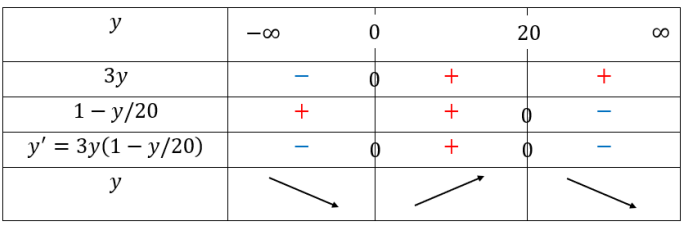
\includegraphics{Images/bifurcation.png}

Which gives us the graph 

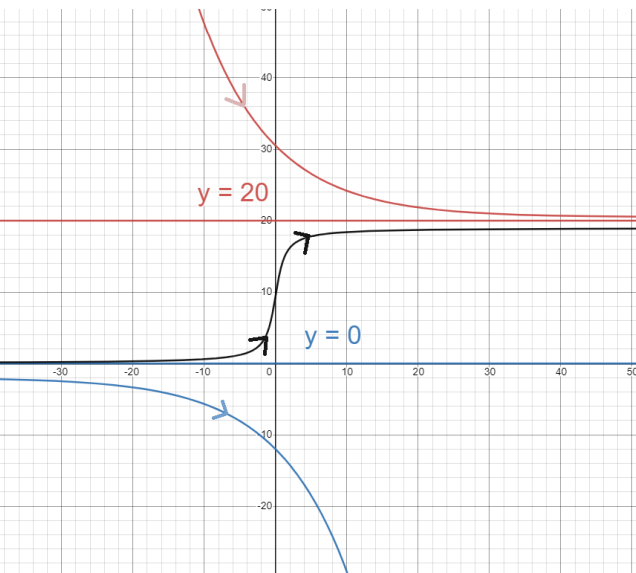
\includegraphics{Images/logistic graph.png}

Classifying solutions:
\begin{itemize}
    \item If the solutions go towards an equilibrium point from each side, it is \emph{stable}
    \item If the solutions move away, it is \emph{unstable}
    \item If the solutions approach from one side and are repelled from the other, it is \emph{bistable}
\end{itemize}

\section{Lecture Sep 14: Existence and uniqueness}
\emph{Existence and Uniqueness Theorem:}
Given $(t_0, y_0)$, consider the ODE 
\[\begin{cases}
    y' = f(y, t)\\
    y(t_0) = y_0
\end{cases}\]
If $f$ and $f_y = \partial f / \partial y$ are continuous near $(t_0, y_0)$, then the ODE has a unique solution $y = y(t)$ for some $t \in (-\delta, \delta), \; \delta > t_0$

Notes:
\begin{itemize}
    \item Because of the uniqueness property, solutions of $y' = f(y, t)$ can never cross
    \item If you only want \emph{existence}, it is enough to assume that $f$ is continuous (you don't need the partial derivative!) 
\end{itemize}

\section{Lecture Sep 16: Separable Equations}
\emph{Separable equation:} an equation in the form 
\[y' = \frac{f(t)}{g(y)}\]

Example 1:
\[\begin{cases}
    t^2 \left(\frac{dy}{dt}\right) = (1 -t^2)(y^2 + 1)\\
    y(1) = 0
\end{cases}\]

Solution:
\[\frac{1}{y^2 + 1} \; dy = \frac{1 - t^2}{t^2} \; dt\]
\[\int \frac{1}{y^2 + 1} \; dy = \int \frac{1}{t^2} - 1 \; dt\]
\[\tan^{-1} y = -\frac{1}{t} - t + C\]
\[y = \tan \left(-\frac{1}{t} - t + C\right)\]
\[0 = \tan (-1 - 1 + C) implies C = 2\]
\[\boxed{y = \tan \left(-\frac{1}{t} - t + 2\right)}\]

Example 2: Solving the logistic equation
\[\begin{cases}
    y' = 3y\left(1 - \frac{y}{20}\right)\\
    y(0) = 10
\end{cases}\]

Solution:
\[\frac{dy}{y (1 - \frac{y}{20})} = 3\; dt\]
\[\int \frac{dy}{y (\frac{20 - y}{20})} = \int 3 \; dt\]
\[\int \frac{20}{y(20 - y)}\; dy = 3t + C\]

To evaluate the left hand side, we must use \emph{partial fractions}:
\[\frac{20}{y(20 - y)} = \frac{A}{y} + \frac{B}{20 - y} = \frac{20A - Ay + By}{y(20 - y)} = \frac{20A + (B - A)y}{y(20 - y)}\]
\[20 = 20A + (B - A)y\]
\[\begin{cases}
    20A = 20\\
    (B - A) = 0
\end{cases} \implies \begin{cases}
    A = 1\\
    B = 1
\end{cases}\]
\[\implies \frac{20}{y (20 - y)} = \frac{1}{y} + \frac{1}{20 - y}\]

Going back to the problem above:
\[\int \frac{20}{y(20 - y)}\; dy = 3t + C\]
\[\int \frac{1}{y} + \frac{1}{20 - y}\; dy = 3t + C\]
\[\ln |y| - \ln |20 - y| = 3t + C\]
\[\ln \left|\frac{y}{20 - y}\right| = 3t + C\]
\[\frac{y}{20 - y} = \pm e^C e^{3t}\]
\[y = Ce^{3t} (20 - y) = 20Ce^{3t} - Cye^{3t}\]
\[y(1 + Ce^{3t}) = 20Ce^{3t}\]
\[\boxed{y = \frac{20Ce^{3t}}{1 + Ce^{3t}}}\]

\section{Lecture Sep 19: Integrating Factors}
To solve equations in the form
\[y' + \alpha y = f(t)\]
multiply by $e^{at}$

Example 1: 
\[\begin{cases}
    3y' = 6y + t\\
    y(0) = 1
\end{cases}\]

Solution:
\[3y' - 6y = t\]
\[y' - 2y = \frac{1}{3}t\]
\[(y' - 2y)e^{-2t} = \frac{1}{3}te^{-2t}\]
\[y'e^{-2t} - 2y e^{-2t} = \frac{1}{3}te^{-2t} \]
\[(y e^{-2t})' = \frac{1}{3}te^{-2t}\]
\[y e^{-2t} = \int \frac{t}{3}e^{-2t}\]
\[y e^{-2t} = \frac{t}{3} \frac{e^{-2t}}{-2} - \int \frac{1}{3} \frac{e^{-2t}}{-2}\; dt \quad \text{(By parts)}\]
\[y e^{-2t} = -\frac{te^{-2t}}{6} - \frac{1}{12}e^{-2t}+C\]
\[\boxed{y = -\frac{t}{6} - \frac{1}{12} + Ce^{2t}}\]

\emph{More general integrating factor:}
For \[y' + P(t) y = f(t)\]
multiply by 
\[e^{\int P(t) dt}\]

Example 2: 
\[y' + 3t^2 y = 6t^2\]

Solution:
\[(y e^{\int 3t^2\; dt})'= 6t^2 e^{\int 3t^2\; dt}\]
\[(y e^{t^3})' = 6t^2 e^{t^3}\]
\[ye^{t^3} = \int 6t^2 e^{t^3} \; dt \quad (u = t^3, 2du = 6t^2\; dt)\]
\[ye^{t^3} = \int 2e^u \; du = 2e^u + C = 2e^{t^3} + C\]
\[y = 2 + Ce^{-t^3}\]

\section{Lecture Sep 21: Exact Equations}
\emph{Exact equation:} equation in the form 
\[P(x, y) \; dx + Q(x, y) \; dy\]

Many ODEs can be reduced to this form:
\[y' = \frac{2xy + y^2}{x^2 + 2xy}\]
\[\implies (x^2 + 2xy) \; dy = -(2xy + y^2) \; dx\]
\[\implies (x^2 + 2xy) \; dy + (2xy + y^2) \; dx = 0\]

Notice, this is the same notation used to solve line integrals in Multivariable calculus!

\emph{Gradient:} If $f = f(x,y)$, then $\nabla f = \langle f_x, f_y \rangle$

To solve, we must find a \emph{potential function} $f$ of $F(x, y)$ such that $F = \nabla f$

Example 1: Find f for $F(x,y) = \langle2xy + y^2, x^2 + 2xy\rangle$
Solution:
\begin{enumerate}
    \item Check that F is conservative
    \[P_y = 2x + 2y\]
    \[Q_x = 2x + 2y\]
    \[P_y = Q_x, \; \therefore F \text{ is conservative}\]
    Because F is conservative, a potential function exists 

    \item Find $f$
    \[F = \nabla f \implies \langle P, Q\rangle = \langle f_x, f_y \rangle\]
    \[f_x = 2xy + y^2 \implies f = \int 2xy + y^2\; dx = x^2y + y^2x + g(y)\]
    \[f_y = x^2 + 2xy \implies f = \int x^2 + 2xy\; dy = x^2 y + xy^2 + f(x)\]

    Collecting all the terms,
    \[f(x, y) = x^2 y + xy^2\]
\end{enumerate}

Amazingly for an ODE 
\[P\; dx = Q\; dy = 0, \quad F = \langle P, Q \rangle\]
the solution is just 
\[f(x, y) = C\]

Therefore, for the example above 
\[x^2y + xy^2 = C\]
(in implicit form)

\emph{Non-exact equations:}
Example 2: $(3xy + y^2) \; dx + (x^2 + xy) \; dy = 0$

Solution:
\[P_y = 3x + 2y\]
\[Q_x = 2x + y\]
So the equation is not exact!

But, we can multiply the ODE by $x$ to get 
\[(3x^2 y + xy^2) \; dx + (x^3 + x^2 y) \; dy = 0\]

In practice, this integrating factor is very difficult to find (requires PDEs) so will be given in this course where necessary. 

Here,
\[P_y = 3x^2 + 2xy\]
\[Q_x = 3x^2 + 2xy\]
\[P_y = Q_x\]

\[f_x = 3x^2 y + xy^2 \implies f = \int 3x^2 y + xy^2 \; dx = x^3 y + \frac{1}{2}x^2 y^2 + g(y)\]
\[f_y = x^3 + x^2 y \implies f = \int x^3 + x^2 y \; dy = x^3 y + x^2 \frac{y^2}{2} + g(x)\]
\[f(x, y) = x^3 y + \frac{1}{2}x^2 y^2\]

Therefore, 
\[\boxed{x^3 y + \frac{1}{2}x^2 y^2 = C}\]

\section{Lecture Sep 28: Numerical Methods I}
\emph{Euler's Method:}
\[y_{n + 1} \approx y_n + h f(y_n, t_n)\]

Given an ODE $y' = f(y, t)$, an initial condition $(t_0, y_0)$, and a number of steps $N$, we can approximate the value of the function at a point by applying the above equation where the step size is  
\[h = \frac{t_n - t_0}{N}\] 

Example 1: Find an approximation of $y(2)$ where 
\[\begin{cases}
    y' = y^2 + 3t\\
    y(0) = 2
\end{cases}\]

Solution:
\[h = \frac{2 - 0}{2} = 1\]
\begin{align*}
    y_0 &= 2\\
    y_1 &= y(0) + f'(2, 0) = 2 + 4 = 6\\
    y_2 &= y(1) + f'(6, 1) = 6 + 39 = 45
\end{align*}

The smaller and more numerous the steps, the more accurate the approximation. 

Indeed, this can be automated via Python computation. 

\section{Lecture Sep 30: Numerical Methods II}
While often good for basic approximations, Euler's method has a number of drawbacks:
\begin{enumerate}
    \item Sensitivity to initial conditions (if there is an exponential term and an issue with rounding, the solution can explode)
    \item Instability (you may need a very small h value to accurately plot a solution, particularly when solutions oscillate)
\end{enumerate}

Alternatives to Euler's method: 
\begin{enumerate}
    \item Backwards Euler:
    \[y_{n+1} = y_n + hf(t_{n + 1}, y_{n + 1})\]
    This is an implicit method that requires knowledge of $y_{n + 1}$

    \item Multistep method 
    \[y_{n+1} = y_n \frac{3}{2}hf(t_n, y_n) - \frac{1}{2}hf(t_{n - 1}, y_{n -1})\] 

    Uses both present and past values of y

    \item Runge-Kutta 
    \[y_{n+ 1} = y_n + hf(t_n + \frac{h}{2}, \; y_n + \frac{h}{2} f(t_n, y_n))\]
    More complicated, but evaluates f at multiple points resolving all other issues
\end{enumerate}

ODEs can also be solved symbolically in Python with the dsolve library in Sympy.

\section{Lecture Oct 3: Systems of ODE I}
Many interactions between objects can be modelled as systems of ODEs which we can represent as matrix equations in the form $\vec{x}' = A\vec{x} + \vec{f}$.

Example 1: 
\[\begin{cases}
    x_1'(t) = 7x_1(t) + 2x_2(t) + t^2\\
    x_2'(t) = -4x_1(t) + x_2(t)
\end{cases}\]
\[\implies \begin{bmatrix}
    x_1'\\
    x_2'
\end{bmatrix} = \begin{bmatrix}
    7 & 2\\
    -4 & 1
\end{bmatrix} \begin{bmatrix}
    x_1\\
    x_2
\end{bmatrix} + \begin{bmatrix}
    t^2\\
    0
\end{bmatrix}\]

\emph{Higher order equations:} Moreover, we can turn any higher order ODE into a system 

Example 2: $y'' + 4y = 0$
Solution:
\[x_1(t) = y, \quad x_2(t) = y'\]
\[\begin{cases}
    x_1' = y' = x_2\\
    x_2' = y'' = -4y = -4x_1
\end{cases}\]
\[\begin{cases}
    x_1' = 0x_1 + x_2\\
    x_2' = -4x_1 + 0x_2
\end{cases}\]
\[\vec{x}(t) = \begin{bmatrix}
    0 & 1\\
    -4 & 0
\end{bmatrix} \vec{x}(t)\]

\section{Lecture Oct 5: Linear Algebra Review}
If for some vector $\vec{v}$, a matrix A, and a scalar value $\lambda$, 
\[A\vec{v} = \lambda\vec{v}\]
then,
$\lambda$ is an \emph{eigenvalue} of A and $\vec{v}$ is an \emph{eigenvector} of A corresponding to $\lambda$

If $\vec{v}$ is an eigenvector, $A\vec{v}$ will lie in its span. 

To find an eigenvalue, solve the equation
\[\det (A - \lambda I) = 0\]

To find the eigenvectors, find the nullspace of $A - \lambda I$: 
\[(A - \lambda I)\vec{v} = \vec{0}\]

\emph{Diagonalization:} a matrix A can be written in the form $A = PDP^{-1}$ where
\[D = \begin{bmatrix}
    \lambda_1 & 0\\
    0 & \lambda_2
\end{bmatrix}, \quad P = \begin{bmatrix}
    \vec{v}_1 & \vec{v}_2
\end{bmatrix}\]\

\section{Systems of ODE II}
The solution of an equation in the form $x' = Ax$ is 
\[x(t) = C_1 \, e^{\lambda_1 t}\; \vec{v}_{\lambda_1} + C_2 \, e^{\lambda_2 t}\; \vec{v}_{\lambda_1}\]

Example 1: Solve $x' = \begin{bmatrix}
    7 & -3\\
    10 & -4
\end{bmatrix}$

Eigenvalues:
\[\begin{vmatrix}
    7 - \lambda & -3\\
    10 & -4 - \lambda
\end{vmatrix} = (7- \lambda)(-4-\lambda) +30 = \lambda^2 - 3\lambda + 2\]
\[(\lambda - 2)(\lambda - 1) = 0 \implies \lambda = \{1, 2\}\]

Eigenvector for $\lambda = 1$:
\[\left[\begin{array}{c c | c}
    6 & -3 & 0\\
    10 & -5 & 0
\end{array} \right]\implies 2x_1 - x_2 = 0\]
\[\vec{v}_{\lambda = 1} = \begin{bmatrix}
    1\\
    2
\end{bmatrix}\]

Eigenvector for $\lambda = 2$:
\[\left[\begin{array}{c c | c}
    5 & -3 & 0\\
    10 & -6 & 0
\end{array}\right] \implies 5x_1 - 3x_2 = 0\]
\[\vec{v}_{\lambda = 2} = \begin{bmatrix}
    3\\
    5
\end{bmatrix}\]

Solution:
\[\boxed{x(t) = C_1 e^{t} \begin{bmatrix}
    1\\2
\end{bmatrix} + C_2 e^{2t} \begin{bmatrix}
    3\\5
\end{bmatrix}}\]

\emph{Phase portraits:}
To draw a phase portrait, solve the system and plot the axes determined by the eigenvectors. On each eigenvector, draw an arrow in the direction of the sign of the eigenvalue for that eigenvector (outwards if positive, inwards if negative). Then, sketch the solutions by drawing lines between the axes according to those arrows.

Example 2: Draw the phase portrait for the curve 
\[x(t) = C_1 e^{-2t} \begin{bmatrix}
    1\\-1
\end{bmatrix}+ C_2 e^{4t} \begin{bmatrix}
    1\\1
\end{bmatrix}\]

Solution:

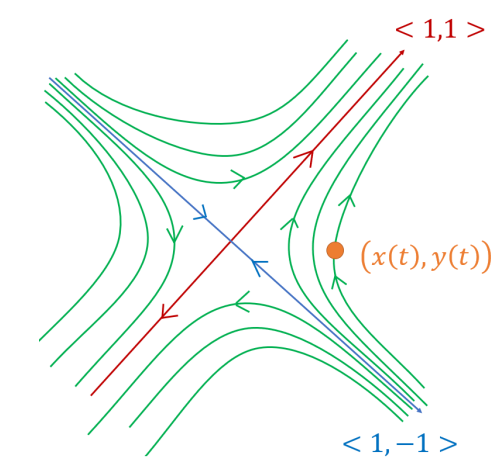
\includegraphics{Images/phase portrait.png}

\section{Oct 12: Complex Eigenvalues}
Remember:
\[i = \sqrt{-1}\]
\[e^{it} = \cos t + i \sin t\]

To solve a system with complex eigenvalues, we need to find a generalized eigenvector. 

Example 1: $x' = \begin{bmatrix}
    -2 & 4\\
    -2 & 2
\end{bmatrix} x$

Here, $\lambda = \pm 2i$

Eigenvector for $\lambda = 2i$:
\[\text{Nul}(A- (2i)I) - \left[\begin{array}{c c | c}
    1 + i & -2 & 0\\
    1 & -1 + i & 0
\end{array}\right]\]
Trick: because we know that $2i$ is an eigenvalue, one of the two rows has to be 0. Choose one and set the other to 0. 
\[\implies \left[\begin{array}{c c | c}
    1 + i & -2 & 0\\
    0 & 0 & 0
\end{array}\right] \implies (1+ i)x_1 -2x_2 = 0\]
\[\vec{v}_{\lambda = 2i} = \begin{bmatrix}
    2\\
    1 + i
\end{bmatrix}\]

Because of the rules of complex conjugates, we don't need the other eigenvector!

Instead, we know that 
\[e^{(2i) t} \begin{bmatrix}
    2\\ 1 +i
\end{bmatrix}\]
is a solution. As we are looking for real solutions, we can use Euler's identity:

\[e^{(2i) t} \begin{bmatrix}
    2\\ 1 +i
\end{bmatrix} = \left(\cos(2t) + i \sin(2t)\right)\left(\begin{bmatrix}
    2\\1
\end{bmatrix} + i \begin{bmatrix}
    0\\1
\end{bmatrix}\right)\]
\[= \left(\cos(2t) \begin{bmatrix}
    2\\1
\end{bmatrix} - \sin(2t) \begin{bmatrix}
    0\\1
\end{bmatrix}\right) + i \left(\cos (2t) \begin{bmatrix}
    0\\1
\end{bmatrix} + \sin(2t) \begin{bmatrix}
    2\\1
\end{bmatrix}\right)\]

So the general solution is 
\[\boxed{x(t) = C_1 \begin{bmatrix}
    2\cos (2t)\\
    \cos(2t) - \sin (2t)
\end{bmatrix} + C_2 \begin{bmatrix}
    2 \sin (2t)\\
    \cos(2t) + \sin(2t)
\end{bmatrix}}\]

To draw a phase portrait, use the principal part of the eigenvector. DO NOT use the generalized eigenvector. The cos and sin terms will then create some kind of elliptical shape where the argument to the trig functions determines if the solution flows clockwise or counterclockwise. 

\section{Lecture Oct 14: Repeated Eigenvalues}
In the case of a single, repeated eigenvalue, find the first eigenvector as normal and then row reduce with that value to find the general. Then, in the final solution, add a correcting factor (which will become clear after studying 2nd order ODEs).

Example 1: $x' = \begin{bmatrix}
    1 & 1\\
    -1 & 3
\end{bmatrix}x$

Eigenvalue:
\[\begin{vmatrix}
    1 - \lambda & 1\\
    -1 & 3 - \lambda
\end{vmatrix} = (1 - \lambda)(3 - \lambda) + 1 = \lambda^2 -4\lambda + 4\]
\[(\lambda - 2)^2 = 0 \implies \lambda = 2\]

Eigenvector for $\lambda = 2$:
\[\left[\begin{array}{c c | c}
    -1 & 1 & 0\\
    -1 & 1 & 0
\end{array}\right] \implies -x_1 + x_2 = 0\]
\[\vec{v}_{\lambda = 2} = \begin{bmatrix}
    1\\1
\end{bmatrix}\]

Generalized eigenvector:
\[(A - 2I)\vec{w} = \begin{bmatrix}
    1\\1
\end{bmatrix}\]
\[\left[\begin{array}{c c |c}
    -1 & 1 & 1\\
    -1 & 1 & 1
\end{array}\right] \implies -x_1 + x_2 = 1\]
\[y = 1 + x\]
\[\vec{x} = \begin{bmatrix}
    x\\
    1 + x
\end{bmatrix} = x \begin{bmatrix}
    1\\1
\end{bmatrix} + \begin{bmatrix}
    0\\1
\end{bmatrix}\]

Solution:
\[\boxed{x(t) = C_1 e^{2t} \begin{bmatrix}
    1\\1
\end{bmatrix} + C_2\left(te^{2t} \begin{bmatrix}
    1\\1
\end{bmatrix} + e^{2t} \begin{bmatrix}
    0\\1
\end{bmatrix}\right)}\]

Note: you are not allowed to rescale the generalized eigenvector

\emph{Plotting phase portraits:} Just like direction fields, phase portraits can be created with a helpful computer program: pplane (https://aeb019.hosted.uark.edu/pplane.html).

Note: when inputting equations into pplane, all multiplications must be explicit (e.g. 3*x not 3x) and no spaces are allowed (e.g. 3+x not 3 + x)

\section{Oct 17: Matrix exponentials}
Notice that equations in the form $x' = Ax$ is analgous to the elementary equation $y' = \alpha y \implies y = Ce^{\alpha t}$. 

Thus, to solve a matrix equation we \emph{can} say that 
\[x = Ce^{At} = Pe^{Dt}P^{-1} \begin{bmatrix}
    C_1\\
    C_2
\end{bmatrix}\]
by the properties of diagonal matrices. 

Example 1: Solve $x' = \begin{bmatrix}
    0 & 1\\
    -2 & 3
\end{bmatrix}$

Eigenvalues:
\[\begin{vmatrix}
    -\lambda & 1\\
    -2 & 3 - \lambda
\end{vmatrix} = \lambda^2 - 3\lambda + 2 = 0\]
\[(\lambda - 1)(\lambda - 2) = 0 \implies \lambda = \{1, 2\}\]

Eigenvector for $\lambda = 1$:
\[\left[\begin{array}{c c |c}
    -1 & 1 & 0\\
    -2 & 2 & 0
\end{array}\right] \implies -x_1 + x_2 = 0\]
\[\vec{v}_{\lambda = 1} = \begin{bmatrix}
    1\\
    1
\end{bmatrix}\]

Eigenvector for $\lambda = 2$:
\[\left[\begin{array}{c c |c}
    -2 & 1 & 0\\
    -2 & 1 & 0
\end{array}\right] \implies -2x_1 + x_1 = 0\]
\[\vec{v}_{\lambda = 2} = \begin{bmatrix}
    1\\
    2
\end{bmatrix}\]

Solution:
\[e^{At} = pe^{Dt}P^{-1}\]
\[ = \begin{bmatrix}
    1 & 1\\
    1 & 2
\end{bmatrix} \begin{bmatrix}
    e^t & 0\\
    0 & e^{2t}
\end{bmatrix} \begin{bmatrix}
    1 & 1\\
    1 & 2
\end{bmatrix}^{-1}\]
\[= \begin{bmatrix}
    2e^t - e^{2t} & -e^t + e^{2t}\\
    2e^t - 2e^{2t} & -e^t + 2e^{2t}
\end{bmatrix}\]

\[\boxed{x(t) = C_1 \begin{bmatrix}
    2e^t - e^{2t}\\
    2e^t - 2e^{2t}
\end{bmatrix} + C_2 \begin{bmatrix}
    -e^t + e^{2t}\\
    -e^t + 2e^{2t}
\end{bmatrix}}\]

\emph{Matrix exponentials with repeated eigenvalues:}
For $2 \times 2$ matrices with one eigenvalue 
\[(A - \lambda I)^2 = 0\]

So, when calculating the Taylor expansion of a matrix exponentiation, all higher terms go to 0. 

So, 
\[e^{At} = e^{\lambda t}e^{(A - \lambda I) t} = e^{\lambda t} \left(I + (A - \lambda I)t\right)\]

Example 2: Solve $x' = \begin{bmatrix}
    -3 & -1\\
    1 & -5
\end{bmatrix}x$

Eigenvalues:
\[\begin{vmatrix}
    -3 - \lambda & -1\\
    1 & -5 - \lambda
\end{vmatrix} = \lambda^2 + 8\lambda + 16\]
\[(\lambda + 4)^2 = 0 \implies \lambda = -4\]

\[e^{At} = e^{-4t}\left(\begin{bmatrix}
    1 & 0\\
    0 & 1
\end{bmatrix} + t\begin{bmatrix}
    1 & -1\\
    1 & -1
\end{bmatrix}\right)\]
\[= e^{-4t} \begin{bmatrix}
    1 + t & -t\\
    t & 1 -t
\end{bmatrix}\]

\[\boxed{x(t) = C_1 e^{-4t} \begin{bmatrix}
    1 + t\\
    t
\end{bmatrix} + C_2 e^{-4t} \begin{bmatrix}
    -t \\
    1- t
\end{bmatrix}}\]

\section{Lecture Oct 19: Nonlinear systems}
For a nonlinear system of interacting $x'$ and $y'$ equations, we can express the system in a form $\vec{x}'(t) = F(\vec{x}(t))$ where:
\[\vec{x}(t) = \begin{bmatrix}
    x(t)\\
    y(t)
\end{bmatrix}, \quad F(x, y) = \begin{bmatrix}
    x'\\
    y'
\end{bmatrix}\]

Recalling the existence-uniqueness theorem, this system will have a unique solution if F and $\nabla F$ are continuous where 
\[\nabla F = \begin{bmatrix}
    \frac{\partial x'}{\partial x} & \frac{\partial x'}{\partial y}\\
    \frac{\partial y'}{\partial x} & \frac{\partial y'}{\partial y}
\end{bmatrix}\]

Example 1: Determine whether a solution exists for 
\[\begin{cases}
    x' = x^2 + xy + e^y\\
    y' = \cos x + 2y
\end{cases}\]

\[F(x, y) = \begin{bmatrix}
    x^2 + xy + e^y\\
    \cos x + 2y
\end{bmatrix}\]
\[\nabla F = \begin{bmatrix}
    2x + y & x + e^y\\
    -\sin x & 2
\end{bmatrix}\]

All these entries are continuous so the ODE has a unique solution for $t$ close enough to 0.

\emph{Classifying equilibrium solutions:}
To classify equilibria, we need to find the linearized systems ($\vec{x}' = \nabla F(\vec{x})$) at those points. To achieve this classification, simply find the eigenvalues of the jacobian at that point.

Example 2: Classify the equilibria of 
\[\begin{cases}
    x' = -x + xy\\
    y' = -8y + 4xy
\end{cases}\]

Solution:
\begin{enumerate}
    \item Find the nullclines 
    \[\begin{cases}
        -x + xy = 0\\
        -8y + 4xy = 0
    \end{cases} \implies \begin{cases}
        x = 0 \text{ or } y = 1\\
        y = 0 \text{ or } x = 2
    \end{cases} \implies (0, 0) \text{ and } (2, 1)\]

    \item Find the linearization
    \[\nabla F = \begin{bmatrix}
        -1 + y & x\\
        4y & -8 + 4x
    \end{bmatrix}\]

    \item Check (0, 0)
    \[\nabla F(0, 0) = \begin{bmatrix}
        -1 & 0\\
        0 & -8
    \end{bmatrix} \implies \lambda = \{-1, -8\}\] 
    So the point (0, 0) is a sink (both are negative)

    \item (This problem finished in the next section)
\end{enumerate}

\section{Lecture Oct 21: Ecology - Competing Species (I)}
\subsection*{Part I - Classifying Equilibrium Points of Nonlinear ODEs}
Example 1: Classify the equilibrium points of
\[\begin{cases}
    x' = -x + xy\\
    y' = -8y + 4xy
\end{cases}\]

To find the equilibrium points, set $x' = 0$ and $y' = 0$

In this equation,
\[\begin{cases}
    x' = -x(1 - y) = 0\\
    y' = -y(8 - 4x) = 0
\end{cases} \implies (0, 0) \quad (2, 1)\]

Linearization:
\[\nabla F(x, y) = \begin{bmatrix}
    \frac{\partial (-x + xy)}{\partial x} & \frac{\partial (-x + xy)}{\partial y}\\
    \frac{\partial (-8y + 4xy)}{\partial x} & \frac{\partial (-8y + 4xy)}{\partial y}\\
\end{bmatrix} = \begin{bmatrix}
    -1 + y & x\\
    4y & -8 + 4x
\end{bmatrix}\]

Case 1: $(0, 0)$
\[\nabla F(0, 0) = \begin{bmatrix}
    -1 & 0\\
    0 & -8
\end{bmatrix}\]

The eigenvalues of this are $\lambda = -1$ and $\lambda = - 8$, both of which are less than zero so the solution is a sink and the point $(0, 0)$ is \textbf{stable}.

Note: For a complex negative eigenvalue (e.g. $\lambda = -2 + 3i$), there will be a spiral sink which is also stable

Case 2: $(2, 1)$
\[\nabla F(2, 1) = \begin{bmatrix}
    0 & 2\\
    4 & 0
\end{bmatrix}\]

Eigenvalues:
\[\lambda^2 - 8 = 0 \implies \lambda = \pm 2\sqrt{2}\]

In this case, one eigenvalue is positive and the other is negative so this is a \textbf{semi-stable saddle point}

Stability cases summary:
\begin{itemize}
    \item If the eigenvalues are both negative, we have a sink
    \item If both positive, unstable
    \item If one positive and one negative, saddle point
    \item If 0, "screwed"
\end{itemize}

\subsection*{Part II - Application Number 1: Competing Species}
Recall: Logistic equation 
\[y' = 3t \left(1 - \frac{y}{20}\right)\]
(the growth of a population with limited resources, where 3 is the growth rate and 20 is the limiting factor)

Guiding question: What if you have two coexisting animal species?
\[\begin{cases}
    x(t) = \text{ population of rabbits}\\
    y(t) = \text{ population of sheep}\\
\end{cases}\]

Note: The two species do not prey on each other but compete for the same limited resources 

\begin{enumerate}
    \item Logistic Approach:
    \[\begin{cases}
        x' = 3x(1 - \frac{x}{1.5})\\
        y' = 2y(1 - \frac{y}{2})
    \end{cases} = \begin{cases}
        x' = 3x - 2x^2\\
        y' = 2y - y^2
    \end{cases}\]
    
    However, this model does not account for competition for limited resources
    
    \item A better model!
    \[\begin{cases}
        x' = 3x - 2x^2 - xy\\
        y' = 2y - y^2 - xy
    \end{cases}\]
    Here, the xy term accounts for the interaction between the two populations 
    (if either were 0, the term would go to zero)
\end{enumerate}

\subsection*{Part III - Equilibria}
Example 2: Find the equilibrium points of the model 
\[\begin{cases}
    x' = x(3 - 2x - y) = 0\\
    y' = y(2 - y - x) = 0
\end{cases}\]

\[\begin{cases}
    x = 0 \implies y = \{0, 2\} \implies \boxed{(0, 0) \quad (0, 2)}\\
    3 - 2x - y = 0 \implies (y = 0 \implies x = \frac{3}{2}) \\
    \text{ OR } \left(2-y-x = 0 \implies \begin{cases}
        3 - 2x - y = 0\\
        2 - y - x = 0
    \end{cases} \implies x = 1, \quad y = 1\right) \implies \boxed{(\frac{3}{2}, 0) \quad (1, 1)}
\end{cases}\]

Thus, the four possible outcomes:
\begin{enumerate}
    \item $(0, 0)$ - Both die 
    \item $(0, 2)$ - Sheep win
    \item $(\frac{3}{2}, 0)$ - Bunnies win 
    \item $(1, 1)$ - Coexistence
\end{enumerate}

To classify each point, we use the linearization:
\[\nabla F(x, y) = \begin{bmatrix}
    \frac{\partial (3x - 2x^2 0 xy)}{\partial x} & \frac{\partial (3x - 2x^2 0 xy)}{\partial y}\\
    \frac{\partial (2y - y^2 - xy)}{\partial x} & \frac{\partial (2y- y^2 - xy)}{\partial y}
\end{bmatrix} = \begin{bmatrix}
    3 - 4x - y & -x\\
    -y & 2 - 2y - x
\end{bmatrix}\]

Thus,
\begin{enumerate}
    \item $F(0, 0) = \begin{bmatrix}
        3 & 0 \\
        0 & 2
    \end{bmatrix} \implies \lambda = \{3, 2\} \implies$ the system is unstable 
    \item $F(0, 2) = \begin{bmatrix}
        1 & 0\\
        -2 & -2
    \end{bmatrix} = \lambda = \{1, -2\} \implies$ the system is semistable so the sheep will survive
    \item $F(\frac{3}{2}, 0) = \begin{bmatrix}
        -3 & -\frac{3}{2}\\
        0 & \frac{1}{2}
    \end{bmatrix} \implies \lambda = \{-3, \frac{1}{2}\} \implies $ the system is also a saddle so the bunnies survive
\end{enumerate}

\section{Lecture Oct 24: Ecology - Competing Species (II)}
\subsection*{Part I - Rabbits and Sheep Model Recap}
Our model, where x is the population of rabbits and y is the population of sheep:
\[\begin{cases}
    x' = 3x - 2x^2 - xy\\
    y' = 2y - y^2 - xy
\end{cases}\]

Equilibrium points: $(0, 0), \; (0, 2), \; (\frac{3}{2}, 0),\; (1, 1)$

\subsection*{Part II - Classification continued}
\[\nabla F(x, y) = \begin{bmatrix}
    3 - 4x - y & -x\\
    -y & 2 - 2y - x
\end{bmatrix}\]
"Again, this is applied math. There is no reason we add this term. It just works. And if it doesn't, we work harder and make up a different term that just works"

\[\nabla F(1, 1) = \begin{bmatrix}
    -2 & -1\\
    -1 & -1
\end{bmatrix}\] 

Eigenvalues:
\[| A - \lambda I | = (-2 - \lambda)(-1 - \lambda) - 1 = \lambda^2 + 3 \lambda + 1 = 0\]
\[\lambda = \frac{-3 \pm \sqrt{9 - 4(1)}}{2} = -\frac{3}{2} \pm \frac{\sqrt{5}}{2}\]

Here, both eigenvalues are negative so (1, 1) is stable

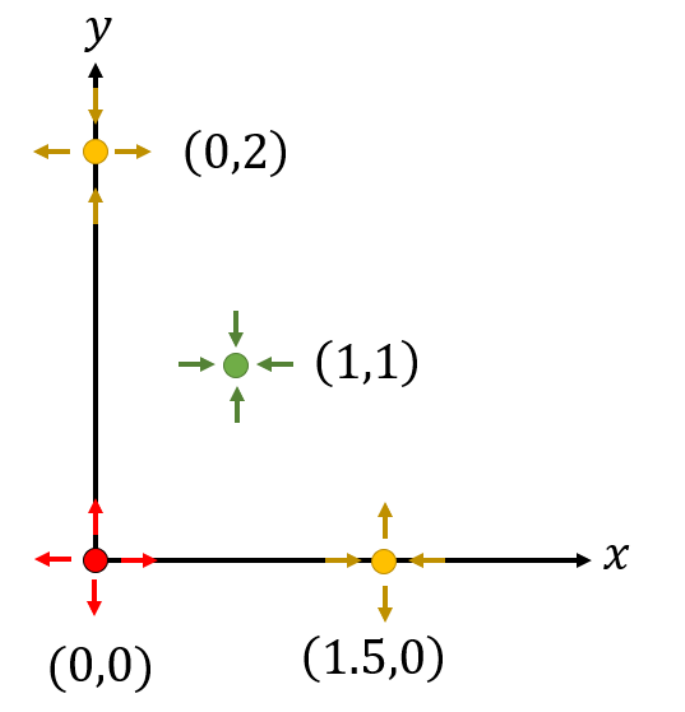
\includegraphics{Images/rabbits and bunnies plot.png}

Note: We do not know which directions of the saddle are positive and which are negative

To draw the rest of the picture, we need to the region $x \in [0, \frac{3}{2}]$ and $y \in [0, 2]$ because those coordinates are the limiting factors of the system 

\subsection*{Part III - Nullclines}
We want to study the behavior of solutions on the axes $x = 0, y = 0, x = 1.5, y = 2$

\emph{Nullclines:} axes where x' or y' is 0

\begin{itemize}
    \item Case 1: $x = 0$ (no rabbits)
        \[\begin{cases}
            x' = 0\\
            y' = 2y - y^2
        \end{cases}\]
        As a result, we are only concerned with vertical movement on the axis.

        Looking at the sign of y', we see that it will be positive $[0, 2]$ and negative $[2, \infty]$

        Therefore, the arrows will be moving up on the y-axis up to 2 and decreasing above 2, so we also now know the orientation of the saddle point.

        Interpretation: if there are no rabbits, the population of sheep will simply increase until they hit their own carrying capacity (which is exactly what we expect!)

    \item Case 2: $y = 0$ (no sheep)
    \[\begin{cases}
        x' = 3x - 2x^2\\
        y' = 0
    \end{cases}\]
    So x will increase until it reaches $x = \frac{3}{2}$

    \item Case 3: $y = 2$ (sheep reached limiting pop)
        \[\begin{cases}
            x' = x - 2x^2\\
            y' = -2x
        \end{cases}\]

        The sign of y' is negative, so on this axis the arrows are pointing down. And, because x' is positive $[0, \frac{1}{2}]$ and negative $[\frac{1}{2}, 1.5]$, the arrows also point roughly towards the centre of the region 

    \item Case 4: $x = 1.5$ (saddle)
        \[\begin{cases}
            x' = - \frac{3}{2}y\\
            y' = \frac{1}{2}y - y^2
        \end{cases}\]

        The sign of x' is negative so the arrows point to the left, and y' is positive on $[0, \frac{1}{2}]$ and negative $[\frac{1}{2}, 2]$
\end{itemize}

From all of this, we can fill in the graph from earlier and draw a few solutions:

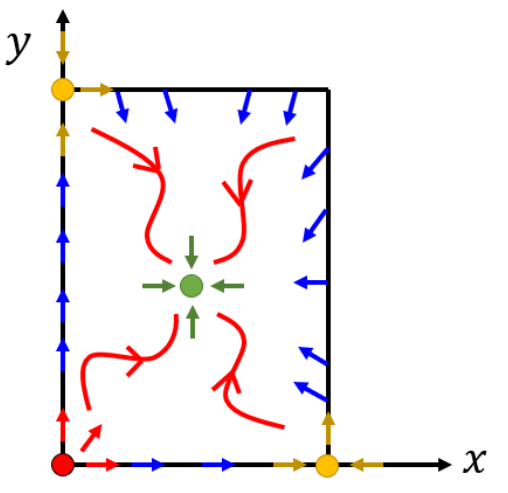
\includegraphics{Images/rabbits and bunnies plot 2.png}

Epic conclusion: the species will not go extinct! they will happily coexist and eventually reach the equilibrium (1, 1)

BUT: we missed the case where there is a periodic orbit around the equilibrium point and where the two species struggle for eternity

\subsection*{Part IV - Periodic Orbits}
To rule out the possibility of periodic orbits, we just need to examine the behavior of the system at the axes of the equilibrium point.

\begin{itemize}
    \item Case 1: $x = 1$
    \[\begin{cases}
        x' = 2x - 2x^2\\
        y' = 1 - x
    \end{cases}\]

    So on the axis $y = 1$, if $x < 1$, the arrows are pointing up, and if $x > 1$, they are pointing down.

    \item Case 2: $y = 1$
    \[\begin{cases}
        x' = 1 -y\\
        y' = -y + y^2
    \end{cases}\]
    So on the axis x = 1, if y < 1, the arrows are pointing to the right (increasing) and if y > 1, they are pointing to the left (x decreasing)
\end{itemize}

Completing the picture, we see that no periodic orbit is possible!

\section{Lecture Oct 26: Midterm Review}
\subsection*{Part I - Chemical Tanks}
Assume there are three chemical tanks in series.
\begin{itemize}
    \item Tank 1: $Q_1(t)$ kg salt, 2L water
    \item Tank 2: $Q_2(t)$ kg salt, 4L water
    \item Tank 3: $Q_3(t)$ kg, 3L water
    \item The first tank has an input of 6L/min of water and 1/3 kg/L salt 
    \item Each minute, 4L salinated water flows from the first tank to the second and from the second to the third
    \item The third tank has an output of 12 L/min
\end{itemize}

Set up a system in the form $Q'(t) = AQ(t) + b$

\begin{enumerate}
    \item $Q'_1(t) = 6 (\frac{1}{3}) - 4 \left(\frac{Q_1(t)}{2}\right) = 2 - 2 Q_1(t)$
    \item $Q_2'(t) = 4 \left(\frac{Q_1(t)}{2}\right) - 4\left(\frac{Q_2(t)}{4}\right) = 2Q_1(t) - Q_2(t)$
    \item $Q_3'(t) = 4\left(\frac{Q_2(t)}{4}\right) - 12\left(\frac{Q_2(t)}{3}\right) = Q_2(t) - 4Q_3(t)$
\end{enumerate}

So, the system is 
\[\begin{cases}
    Q_1' = -2Q_1 + 2\\
    Q_2' = 2Q_1 - Q_2
    Q_3' = Q_2 - 4Q_3
\end{cases}\]

So,
\[Q' = \begin{bmatrix}
    -2 & 0 & 0\\
    2 & -1 & 0\\
    0 & 1 & -4
\end{bmatrix} Q(t) + \begin{bmatrix}
    2\\0\\0
\end{bmatrix}\]

\subsection*{Part II - Matrix Exponentials}
Example 2: Use matrix exponentials to solve $x' = Ax$ where 
\[A = \begin{bmatrix}
    7 & -1\\
    9 & 1
\end{bmatrix}, \quad x(0) = \begin{bmatrix}
    2\\3
\end{bmatrix}\]

Solution:
\[\begin{vmatrix}
    7 - \lambda & -1\\
    9 & 1 - \lambda
\end{vmatrix} = (7 - \lambda)(1 - \lambda) + 9 = \lambda^2 - 8\lambda + 16 = 0\]
\[(\lambda - 4)^2 = 0 \implies \lambda = 4\]

\[e^{At} = e^{4t} e^{(A - 4I)t} = e^{4t} (I + (A - 4I)t)\]
\[e^{4t} \left(\begin{bmatrix}
    1 & 0\\
    0 & 1
\end{bmatrix} + t\begin{bmatrix}
    3 & -1\\
    9 & -3
\end{bmatrix}\right)\]
\[= e^{4t} \begin{bmatrix}
    1 + 3t & -t\\
    9t & 1 - 3t
\end{bmatrix}\]

\[x(t) = C_1 e^{4t} \begin{bmatrix}
    1 + 3t\\
    9t
\end{bmatrix} + C_2 e^{4t} \begin{bmatrix}
    -t\\
    1 - 3t
\end{bmatrix}\] 

\[x(0) = \begin{bmatrix}
    2\\3
\end{bmatrix} = C_1\begin{bmatrix}
    1\\
    0
\end{bmatrix} + C_2 \begin{bmatrix}
    0\\1
\end{bmatrix} \implies C_1 = 2, \quad C_3 = 3\]

\[x(t) = 2e^{4t}  \begin{bmatrix}
    1 + 3t\\
    9t
\end{bmatrix} + 3e^{4t} \begin{bmatrix}
    -t\\
    1 - 3t
\end{bmatrix} = \boxed{e^{4t} \begin{bmatrix}
    2 + 3t\\
    3 + 9t
\end{bmatrix}}\]

\subsection*{Part III - Euler's Method}
Example 3: Apply Euler's method with N = 2 to find $y_0, y_1, y_2$ on $[2, 6)$ where
\[\begin{cases}
    y' = y^2 - 2t\\
    y(2) = 1
\end{cases}\]

Solution:
\[h = \frac{6 - 2}{2} = 2\]
\begin{align*}
    y_0 = 1\\
    y_1 = y_0 + h y'(2) = 1 + 2 (1 - 4) = -5\\
    y_2 = y_1 + h y'(4) = -5 + 2 (25 - 8) = -5 + 34 = 29
\end{align*}

\subsection*{Part IV - Phase Portraits}
Example 4: Sketch the phase portrait of $x' = Ax$ where
\[A = \begin{bmatrix}
    3 & 4\\
    -1 & 3
\end{bmatrix}\]

Solution:
\[\lambda = 3 \pm 2i\]
\[\vec{v}_{3 + 2i} = \begin{bmatrix}
    -2i\\
    1
\end{bmatrix}\] 

\[e^{(3 + 2i)t} \begin{bmatrix}
    -2i\\
    1
\end{bmatrix} = e^{3t} \left(\cos (2t) + i \sin (2t)\right) \left(\begin{bmatrix}
    0\\
    1
\end{bmatrix} - i \begin{bmatrix}
    2\\0
\end{bmatrix}\right)\]

\[x(t) = C_1 \left(e^{3t} \cos (2t) \begin{bmatrix}
    0\\1
\end{bmatrix} + \sin(t) \begin{bmatrix}
    2\\0
\end{bmatrix}\right) + C_2 e^{3t} \left(\cos(2t) \begin{bmatrix}
    -2\\
    0
\end{bmatrix} + \sin (2t) \begin{bmatrix}
    0\\1
\end{bmatrix}\right)\]

\section{Lecture Oct 31: Epidemiology - SIR Models (I)}
\emph{Epidemiology:} study of infectious diseases 
Questions to be solved with ODEs;
\begin{itemize}
    \item How does COVID-19 spread?
    \item When do poutbreaks occur?
    \item How to "flatten the curve"?
    \item How to prevent outbreaks?
\end{itemize}

\subsection*{Part I - SIR model}
S is "susceptible" (those exposed to COVID)
I is "infected" (assuming that those who are infected can immediately infect others)
R is "recovered" (assume that once recovered, cannot get it again)

We choose a "compartmental model" where people transition between the three SIR states.

Constant assumptions:
\begin{itemize}
    \item The constant rate of flow from I to R, $\gamma$
    \item The mean residence time $1/ \gamma$ (the average time for a person to recover)
    \item The "turnover rate" where susceptible people become infected (S to I), $\left(\frac{b}{N}\right) I$
        where $N = S + I + R$ (the total population) and b is the number of people an infected person infects
\end{itemize}

The system:
\[\begin{cases}
    S'(t) = 0 - \left(\frac{b}{N}\right) SI\\
    I'(t) = \left(\frac{b}{N}\right) SI - \gamma I\\
    R'(t) = \gamma I
\end{cases}\]

The SI cross terms make this nonlinear. 

Notice that 
\[N' = (S + I + R)' = 0\]
so the total population is constant. This matters because you only need to solve two of the equations to find the third ($R = N - S - I$). 

Reduced model:
\[\begin{cases}
    S' = -\left(\frac{b}{N}\right) SI\\
    I' = \left(\frac{b}{N}\right) SI - \gamma I
\end{cases}\]

\subsection*{Part II - Rescaling Time}
"A day is just a social construct... more or less."

To even further simplify the model, we can define a new time for which $\tau = 1 \implies t = \frac{1}{\gamma}$ so 
\[\tau = \gamma t\]
and define x and y to be $\frac{S}{N}$ and and $\frac{I}{N}$

This gives:
\[\begin{cases}
    x(\tau) = \frac{S(t)}{N} = \frac{S(\tau / \gamma)}{N} \implies S(t) = Nx(\tau) = Nx(\gamma t)\\
    y(\tau) = \frac{I(t)}{N} = \frac{I(\tau / \gamma)}{N} \implies I(t) = Nx(\tau) =  Ny(\gamma t)
\end{cases}\]

So the new model is:
\[\begin{cases}
    S' = (Nx(\gamma t))' = N' x(\gamma t) + N\gamma x'(\gamma t) = \gamma N x'(\tau)
    -\frac{b}{N} SI = \frac{-b}{N}(Nx)(Ny) = -bNxy\\
    I' = (Ny(\gamma t))' = N' y(\gamma t) + N\gamma y'(\gamma t) = \gamma N y'(\tau)\\
    \frac{b}{N} - \gamma I = \frac{b}{N}(Nx)(Ny) - \gamma Ny = bNxy - Ny
\end{cases}\]
\[\implies \begin{cases}
    x' = \left(\frac{-b}{\gamma}\right)xy\\
    y' = \left(\frac{b}{\gamma}\right)xy - y\\
\end{cases}\]

We then define $R_0 = b / \gamma$ as the total number of people a sick person ingects

So, at long last, 
\[\boxed{\begin{cases}
    x' = -R_0 xy\\
    y' = R_0 xy - y
\end{cases}}\]

\subsection{Lecture Nov 2:  Epidemiology - SIR Models (II)}
\subsection*{Part I - Recap SIR Model}
After making some simplifications and several changes of variable, we have the model

\[\begin{cases}
    x' = -R_0 xy\\
    y' = R_0 xy - y
\end{cases}\]
Where x is the fraction of sus people, y is fraction of infected people, $R_0$ is number of people a sick person infects while sick

\subsection*{Part II - Equilibrium points ($x' = 0, y' = 0)$}
\[\begin{cases}
    -R_0 xy = 0\\
    R_0 xy - y = 0
\end{cases} = \begin{cases}
    xy = 0\\
    y(R_0 x - 1) = 0
\end{cases} \implies \begin{cases}
    x = 0 \; \text{ OR } \; y = 0\\
    \text{ if } x = 0 \implies y = 0\\
    \text{ if } y = 0 \implies 0 (R_0 x - 1) = 0 
\end{cases}\]

This second equation implies that there are infinitely many equilibria of the form $(x, 0)$

Interpretation: our equilibrium solution is the point where no one is infected 

\subsection*{Part III - Classification}
\[\nabla F(x, y) = \begin{bmatrix}
    -R_0 y & -R_0 x\\
    R_0 y & R_0 x - 1
\end{bmatrix}\]
\[\nabla F(x, 0) = \begin{bmatrix}
    0 & -R_0 x\\
    0 & R_0 x - 1
\end{bmatrix}\]

This is upper triangular so the eigenvalues are $\lambda = 0$ (neutral) and $\lambda = R_0 x - 1$ (sometimes positive and negative)

From the eigenvalue:
\[\lambda = R_0 x - 1 \implies x = \frac{1}{R_0}\]
\[\begin{cases}
    \lambda < 0 \quad x < \frac{1}{R_0}\\
    \lambda > 0 \quad x > \frac{1}{R_0}
\end{cases}\]

Conclusion:
\[(x, 0) \; \text{ is } \; \begin{cases}
    \text{Stable} \quad x < \frac{1}{R_0}\\
    \text{Unstable} \quad x > \frac{1}{R_0}
\end{cases}\]

\subsection*{Part IV - The Good Case ($R_0 < 1$)}
If $R_0 < 1 \implies 1/R_0 > 1$
However, because x and y are defined as fractions of the population, we will never reach that point so all equilibrium solutions will be stable. 
In other words, no matter what, the number of infected people will eventually go to 0

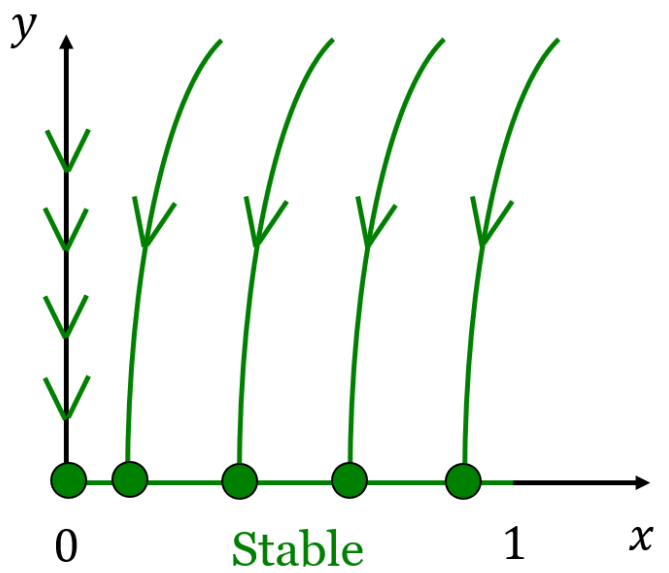
\includegraphics{Images/sir stability.png}

\subsection*{Part V - The Bad Case ($R_0 > 1$)}
On the right hand side of $1/R_0$, all equilibrium solutions are unstable while on the left they are stable so we get outbreaks!

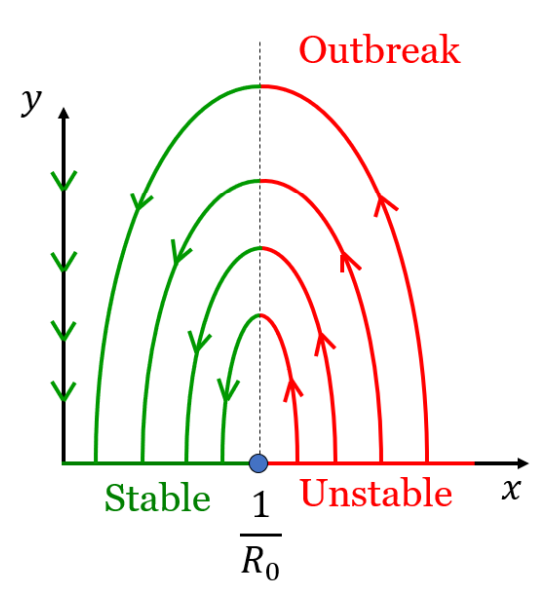
\includegraphics{Images/sir outbreak.png}

This makes sense because $R_0$ is the number of people a sick person infects. If this is high, a sick person infects many people which causes an exponential infection tree leading to a pandemic.

To find the arrows on the phase portrait, we just see that
\[\begin{cases}
    x' = -R_0 xy < 0 \implies  \text{arrows go left}\\
    y' = y(R_0 x - 1) \implies \text{positive when right of $1/R_0$, negative otherwise}
\end{cases}\]

\subsection*{Part VI - Vaccines}
Definition: $z = \frac{R}{N}$,  the fraction of recovered/vaccinated people 

Notice that $x + y + z = 1$ 
If $z > 1 - \frac{1}{R_0}$ then $x < \frac{1}{R_0}$ and no outbreaks!
"If enough people are vaccinated, then there will be no outbreak"

\subsection*{Part VII - Real COVID Data (Spring 2020)}
NYT says $R_0 \approx 3.8$ 
so 
\[1 - \frac{1}{R_0} \approx 0.74\]
Therefore, in order to control COVID, 74\% of the population needs to be vaccinated. 

According to Google, 68\% of people are currently vaccinated

\section{Lecture Nov 4: 2nd Order ODEs (I)}
\subsection*{Part I - Existence and Uniqueness}
Example 1:
\[\begin{cases}
    y'' = 2y' + t(y^2)\\
    y(0) = 2\\
    y'(0) = 3
\end{cases}\]

\emph{Existence and Uniqueness for 2nd Order:} Given $y_0$ and $v_0$, for 
\[\begin{cases}
    y'' = f(y, y', t)\\
    y(0) = y_0\\
    y'(0) = v_0
\end{cases}\]
If f and its partial derivatives are continuous, there is a unique solution $y = y(t)$ near 0

\subsection*{Part II - Model Problem}
Example 2: 
Solve $y'' - 5y' + 6y = 0$

Recall: $y' = ry \implies y = Ce^{rt}$

Plug in $e^{rt}$:
\[(e^{rt})'' - 5(e^{rt})' = 6(e^{rt}) = 0\]
\[r^2e^{rt} - 5re^{rt} + 6e^{rt} = 0\]
\[(r^2 - 5 + 6) e^{rt} = 0\]
\[(r - 3)(r - 2) = 0 \implies r = \{3, \; 2\}\]
So, $e^{2t}$ and $e^{3t}$ are solutions

In this case, $r^2 - 5r + 6 = 0$ is the \emph{auxiliary equation}

General Solution:
\[y = Ae^{2t} + Be^{3t}\]

Why does this work?
\begin{itemize}
    \item From $r = \{2, \; 3\}$ we know that $e^{2t}$ and $e^{3t}$ are solutions
    \item A constant times a solution is still a solution
    \item So $Ae^{2t}$ and $Be^{3t}$ are also solutions 
    \item The sum of solutions is still a solution (the solution space is the span of the basis vectors $e^{2t}$ and $e^{3t}$)
    \item Using $y(0)$ and $y'(0)$, you can solve for A and B
    \item By uniqueness, $y = Ae^{2t} + Be^{3t}$
\end{itemize}

\subsection*{Part III - Examples}
Example 3: $y'' + 5y' + 4y = 0$

Solution:
We can go directly to the auxiliary equation
\[r^2 + 5r + 4 = 0\]
\[(r + 4)(r + 1) = 0 \implies 4 = \{-4, \; -1\}\]
\[\boxed{y} = Ae^{-t} + Be^{-4t}\]

Example 4: $4y'' = 8y' - 3y$

Solution:
\[4r^2 - 8r + 3 = 0\]
\[(2r - 3)(2r - 1) = 0 \implies r = \{\frac{3}{2}, \; \frac{1}{2}\}\]

\[\boxed{y = Ae^{3t/2} + Be^{t/2}}\]

Example 5:
\[\begin{cases}
    y'' + y' - 6y = 0\\
    y(0) = 2\\
    y'(0) = -1
\end{cases}\]

Solution:
\[r^2 + r - 6 = 0\]
\[(r + 3)(r - 2) = 0 \implies r = \{-3, \; 2\}\]
\[y = Ae^{-3t} + Be^{2t}\]

\[y(0) = 2 \implies A + B = 2\]
\[y' = -3Ae^{-3t} + 2Be^{2t}\]
\[y'(0) = -1 \implies -3A + 2B = -1\]
\[\begin{cases}
    A + B = 2\\
    -3A + 2B = -1
\end{cases} \implies -3A + 2(2 - A) = -1\]
\[-5A = -5 \implies A = 1, \; B = 1\]
\boxed{y = e^{-3t} + e^{2t}}


Example 6: When does this attain a min?
\[y = e^{-3t} + e^{2t}\]

Solution:
Set $y' = 0$:
\[(e^{-3t} + e^{2t})' = 0\]
\[-3e^{-3t} + 2e^{2t} = 0 \implies 2e^{2t} = 3e^{3t}\]
\[e^{5t} = \frac{3}{2}\]
\[t = \frac{1}{5} \ln \frac{3}{2} \approx 0.081\]

(Then technically you should also check the 2nd derivative)

Example 7: $y''' - 6y'' + 11y' - 6y = 0$

Solution:
\[r^3 - 6r^2 + 11r - 6 = 0\] 
\[(r - 1)(r - 2)(r - 3) = 0\]
\[r = \{1,\; 2,\; 3\}\]
\boxed{y = Ae^{t} + Be^{2t} + Ce^{3t}}

\section{Lecture Nov 7: 2nd Order ODEs (II)}
\subsection*{Part I - Complex roots}
Example 1: $y'' + y = 0$

Solution:
\[r^2 + 1 = 0 \implies r = \pm i \]

From "our buddy" Euler:
\[y = Ce^{it} = \cos t + i \sin t\]

So, 
\[y = A\cos t + B \sin t\]

Example 2: 
\[\begin{cases}
    y'' + 4y = 0\\
    y(0) = 3\\
    y'(0) = 4
\end{cases}\]

Solution:
\[r^2 + 4 = 0 \implies r^2 = -4 \implies r = \pm 2i\]
\[y = A\cos(2t) + B\sin (2t)\]
\[y(0) = A  = 3\]
\[y'(0) = -2A \sin(2(0)) + 2B\cos (2(0)) = 2B = -4 \implies B = -2\]
\boxed{y = 3\sin(2t) -2 \cos(2t)}

Example 3: $y'' - 4y' + 13y = 0$
\[r^2 - 4r + 13 = 0\]
\[r = \frac{4 \pm \sqrt{16 - 4(13)}}{2} = 2\pm 3i\]
\[y = e^{2t} (A\cos(3t) + B\sin(3t))\] 
\boxed{y = Ae^{2t} \cos (3t) + Be^{2t} \sin (3t)}

\subsection*{Part II - Repeated roots}
Example 4: $y'' - 4y' + 4y = 0$
\[(r - 2)^2 = 0 \implies r = 2 \text{ (repeated)}\]

FACT: $y = Ae^{2t} + Bte^{2t}$

\emph{Why this is true:} 
\[\left(e^{-2t} y\right)'' = 0\]
\[\left(e^{-2t} y \right)' = B\]
\[e^{-2t} y = Bt + A\]
\[y = Ae^{2t} + Bte^{2t}\]

\section{Lecture 9 November: Boundary Value Problems}
\subsection*{Part I - Boundary Value Problems}
Example 1: Find the value of $\lambda$ for which the following has a zonzero solution:
\[\begin{cases}
    y'' = \lambda y\\
    y(0) = 0\\
    y(\pi) = 0
\end{cases}\]

Solution:
\[r^2 = \lambda\]

Case 1 $\lambda > 1$: Then $\lambda = \omega^2$ for some $\omega > 0$
Then, the auxiliary equation is 
\[r^2 = \omega^2 \implies r = \pm \omega\]
\[y = Ae^{\omega t} + Be^{-\omega t}\]
\[y(0) = A + B = 0 \implies B = - A\]
\[y(\pi) = Ae^{\omega \pi} - Ae^{-\omega \pi} \implies Ae^{\omega \pi} = A e^{-\omega \pi}\]
$A \neq 0$ because we are looking for nonzero solutions so 
\[e^{\omega \pi} = e^{-\omega \pi}\]
\[\omega = 0 \implies \lambda = 0\]
So, there are no nonnegative solutions here!

Case 2: $\lambda = 0$: 
Aux: 
\[r^2 = 0 \implies r = 0\]
\[y = A + Bt\]
\[y(0) = A = 0\]
\[y(\pi) = B\pi = 0 \implies B = 0\]
\[y = 0\]
So no nonzero solutions here either!

Case 3: $\lambda < 0$
Then 
\[\lambda = -\omega^2 \quad (\omega > 0)\]
Aux:
\[r^2 = \lambda = -\omega^2 \implies r = \pm \omega i\]
\[y = A\cos (\omega t) + B \sin (\omega t)\]
\[y(0) = A = 0\]
\[y = B\sin (\omega t)\]
\[y(\pi) = B\sin (\omega \pi) = 0\]
B cannot be zero (or it would be the zero solution yet again)
\[\sin (\omega \pi) = 0\]
\[\omega \pi = \pi m\]
\[\omega = m\]
Where m is any positive integer so:
\[\begin{cases}
    \lambda = -\omega^2 = -m^2\\
    y = B \sin (\omega t) = B \sin(m t)
\end{cases}\]

Epic conclusion:
\begin{enumerate}
    \item Eigenvalues are $\lambda = -m^2, \quad m \in \mathbb{Z}^+$
    \item Eigenfunctions: $y = \sin (mt)$ (this is the basis for the solution space)
\end{enumerate}

\subsection*{Part II - Derivative Example}
Example 2: Find the eigenvalues/functions of 
\[\begin{cases}
    y'' = \lambda\\
    y'(0) = 0\\
    y'(1) = 0
\end{cases}\] 

Auxiliary equation:
\[r^2 = \lambda\]

Case 1: $\lambda > 1$
\[r^2 = \lambda = \omega^2 \implies r = \pm \omega\]
\[y = Ae^{\omega t} + Be^{-\omega t}\]
\[y' = A\omega e^{\omega t} -B\omega e^{-\omega t} \]
\[y'(0) = A\omega -B\omega\]
$\omega$ is positive so we can cancel it and we have $A= B$
\[y'(1) = A\omega e^\omega - A\omega e^{-\omega} = 0 \implies \omega = -\omega \implies \omega = 0\]
This is a contradiction so there are no nonzero solutions

Case 2: $\lambda = 0$
\[r^2 = 0 \implies r = 0\]
\[y = A + Bt\]
\[y' = B\]
\[y'(0) = 0 \implies B = 0\]
\[y = A\]
\[y' = 0\]
So $\lambda = 0$ is an eigenvalue with eigenfunction $y = A$ 

Case 3: $\lambda < 0$
\[\lambda = -\omega^2 \quad (\omega > 0)\]
\[r^2 = \lambda \implies r = \pm \omega i\]
\[y = A \cos (\omega t) + B \sin (\omega t)\]
\[y' = -A \omega \sin (\omega t) + B \omega \cos (\omega t) \]
\[y'(0) = B \omega = 0 \implies B = 0\]
\[y = A \cos (\omega t)\]
\[y'(1) = -A\omega \sin (\omega) = 0\]
\[\sin (\omega) = 0 \implies \omega = \pi m \]

So the eigenvalues are $\lambda = -(\pi m)^2 \quad m \in \mathbb{Z}^+_0$ for the eigenfunctions $y = \cos (\pi m t) \quad m \in \mathbb{Z}^+$

\section{Lecture Nov 11: Undetermined Coefficients}
\subsection*{Part I - Inhomogeneous Equations}
Example 1: $y'' - 5y' + 6y = e^t$

Solution:
\begin{enumerate}
    \item Homogeneous solution (solve $y'' - 5y' + 6y = 0$)
    \[r^2 - 5r + 6 = (r - 3)(r - 2) = 0 \implies y_0 = Ae^{3t} + Be^{2t}\]
    \item Particular solution (find \emph{one} solution to $y'' - 5y' + 6y = e^t$)
    \[y_p(t) = \frac{1}{2}e^t\]
    \item Final answer:
    \[y = y_0 + y_p\]
    So, 
    \[y = Ae^{3t} + Be^{2t} + \frac{1}{2}e^t\]
\end{enumerate}

Why this works:
$y - y_p$ solves $y'' - 5y' + 6y =9 \implies y- y_0 = y_0$

\subsection*{Part II - Undetermined coefficients}
Example: Find a particular solution $y_p$ of $y'' - 5y' + 6y = e^t$

Some heuristic solutions:
\begin{itemize}
    \item If RHS is $e^{rt}$, guess $y_p = Ae^{rt}$
    \item IF RHS is a polynomial, guess $y_p$ to be the most general polynomial of the same degree 
    (e.g. $t^2 \longrightarrow At^2 + Bt + C$)
    \item $\cos$ always goes with $\sin$
    (e.g. $\cos(\alpha t) \longrightarrow A\cos(\alpha t) + B\sin(\alpha t)$)
\end{itemize}

In the above problem,
\[(Ae^t)'' - 5(Ae^t)' + 6Ae^= e^t\]
\[Ae^t - 5Ae^t + 6Ae^t = e^t \implies 2Ae^2 = e^t\]
\[A = \frac{1}{2}\]
So, 
\[y_p = \frac{1}{2}e^t\]

Example 3 (Rule 2 above):
Find the general solution of $y'' - 2y' - 3y = 9t^2$

Homogeneous Solution:
\[r^2 - 2r - 3 = 0 = (r - 3)(r + 1) \implies y = Ae^t + Be^{3t}\]

Particular solution:
\[\text{RHS} = 9t^2\] 
\[y_p = At^2 + Bt + C\]
\[(At^2 + Bt + C)'' - 2(At^2 + Bt + C)' - 3(At^2 + Bt + C) = 9t\]
\[2A - 2(2At + B) - 3(At^2 + Bt + C) = 9t^2\]
\[2A - 4At - 2B - 3At^2 - 3Bt -3C = 9t^2\]
\[-3At^2 + (-4A - 3B)t + (2A - 2B - 3C) = 9t^2\]
\[\begin{cases}
    -3A = 9 \implies A = -3\\
    -4A - 3B = 0 = -4(-3) - 3B = 0 \implies B = 4\\
    2A - 2B - 3C = 0 = 2(-3) - 2(4) - 3C = 0 \implies C = -14/3
\end{cases}\]
\[y_p = -3t^2 + 4t - \frac{14}{3}\]

General solution:
\[y = y_0 + y_p = \boxed{Ae^{3t} + Be^{-t} - 3t^2 + 4t - \frac{14}{3}}\]

Example 4 (rule 3 above):
\[\begin{cases}
    y'' - y' = \cos (2t)\\
    y(0) = 2 \quad y'(0) = -1
\end{cases}\]

Homogeneous:
\[r^2 - r = 0 \implies y = A + Be^t\]

Particular:
\[\text{RHS} = \cos (2t)\]
\[y_p = A\cos(2t) + B\sin(2t)\]
\[(A\cos(2t) + B\sin(2t))'' - (A\cos(2t) + B\sin(2t))' = \cos (2t)\]
\[-4A\cos(2t) -4B\sin(2t) + 2A\sin(2t) - 2B\cos (2t) = \cos (2t)\]
\[(-4A - 2B)\cos(2t) + (-4B + 2A)\sin(2t) = 1\cos(2t) + 0\sin(2t)\]
\[\begin{cases}
    -4A - 2B = 1\\
    2A - 4B = 0\end{cases} \implies A = -\frac{1}{5}\quad B = -\frac{1}{10}\]
\[y_p = -\frac{1}{5}\cos(2t) - \frac{1}{10}\sin (2t)\]

General solution:
\[y = A + Be^t - \frac{1}{5} \cos (2t) - \frac{1}{10} \sin (2t)\]

Initial conditions:
\[A + B - \frac{1}{5} = 2\]
\[y' = Be^t + \frac{2}{5}\sin (2t) - \frac{1}{5}\cos (2t)\]
\[B - \frac{1}{5} = -1 \implies B = -\frac{4}{5} \implies A = 3\]
\[\boxed{y} = 3 - \frac{4}{5}e^t - \frac{1}{5} \cos (2t) - \frac{1}{10}\sin(2t)\]

\subsection*{Part III - Resonance}
Example 5: $y'' - 5y' + 6y - e^{2t}$

Homogeneous solution:
\[r^2 - 5r + 6 = 0 \implies y_0 = Ae^{2t} + Be^{3t} \]

Particular solution:
Naively, $y_p = Ae^{2t}$
But!
\[(Ae^{2t})'' - 5(Ae^{2t})' + 6(Ae^{2t}) = 4Ae^{2t} - 10Ae^{2t} + 6Ae^{2t} = 0 \neq e^{2t}\]
Because this guess is already part of the homogeneous solution, we need a new particular solution!

In other words, if the root of the particular solution coincides with the homogenous solution, we add a resonance term:
\[y_p = Ate^{2t}\]

\[(Ate^{2t})'' - 5(Ate^{2t})' + 6(Ate^{2t}) = e^{2t} \implies A = -1\]
\[y_p = -te^{2t}\]
\[\boxed{y = Ae^{2t} + Be^{3t} - te^{2t}}\]

Example 6: Guess the form of $y_p$
\begin{enumerate}
    \item $y'' + 3y' - 4y = e^{2t}$
    Aux $r^2 + 3r - 4 = 0 \implies r = \{1, \; -4\}$ but $e^{2t} \implies r = 2$ so the roots do not coincide, and there is no resonance
    \boxed{y_p = Ae^{2t}}
    \item $y'' + 3y' - 4y = e^{t}$
    $e^{t} \implies r = 1$ which corresponds to the root of the aux equation so 
    \boxed{y_p = Ate^t}
    \item $y'' - 3y' -4y = t^2 e^{-4t}$
    $t^2 e^{-4t} \implies r = -4$ so there is still resonance and 
    \boxed{y_p = t(At^3 + Bt^2 + Ct + D) e^{-4t}}
\end{enumerate}

\section{Lecture Nov 14: Mechanical Vibrations}
\subsection*{Part I - Masses and Springs}
Image a mass suspended below a spring where $y(t)$ is the displacement from the equilibrium position

\[my'' + \gamma y' + Ky = F\]
Where:
\begin{itemize}
    \item M is mass
    \item $\gamma$ is a damping constant (friction)
    \item K is a spring constant 
    \item F is the external force
\end{itemize}

Notes on the derivation:
\begin{itemize}
    \item $my''$ comes from $F = ma$
    \item $\gamma y'$ is the damping force and also comes from Newton
    \item $Ky$ comes from Hooke's law 
    \item F is just external forces
\end{itemize}

\subsection*{Part II - Free vibrations}
Example 1:
\[\begin{cases}
    2y'' + 18y = 0\\
    y(0) = 2\\
    y'(0) = 6\sqrt{3}\\
    \gamma = 0, \quad F = 0
\end{cases}\]

\begin{enumerate}
    \item Aux: $2r^2 + 18 = 0 \implies r = \pm 3i$
    \item $y = A\cos(3t) + B\sin(3t)$
    \item $A = 2 \quad B = 2\sqrt{3}$
    \item $\boxed{y = 2\cos(3t) + 2\sqrt{3} \sin (3t)}$
\end{enumerate}
This looks like a sine wave with frequency $\omega = 3$, period $T = \frac{2\pi}{3}$, amplitude $R = \sqrt{A^2 + B^2} = 4$, phase shift $\delta = \tan^{-1} \left(\frac{B}{A}\right) = \frac{\pi}{3}$
From precalc,
\[y = R\cos(\omega t - \delta) = 4\cos(3t - \frac{\pi}{3})\]

\subsection*{Part III - Damping}
Example 2:
\[\begin{cases}
    9y'' + 6y' + 37y = 0\\
    y(0) = 4\\
    y'(0) = -2
\end{cases}\]

Solution:
\[9r^2 + 6r + 37 = 0\]
\[r = \frac{-6 \pm \sqrt{-1296}}{18} = -\frac{1}{3} \pm 2i\]
\[y = Ae^{-t/3}\cos(2t)+ Be^{-t/3} \sin(2t)\]
\[A = 4 \quad B = -\frac{1}{3}\]
\[y = 4e^{-t/3}\cos(2t)- \frac{1}{3} e^{-t/3} \sin(2t)\]

Notice that
\[\lim_{t \to \infty} y = 0\]

\subsection*{Part IV: Forcing}
Example 3: 
\[\begin{cases}
    y'' + 4y = 5\cos(3t)\\
    y(0) = 1\\
    y'(-4)
\end{cases}\]

Solution:
\begin{enumerate}
    \item Homogeneous solution $y'' + 4y = 0$
    \[y_0 (t) = A \cos(2t) + B \sin(2t)\] 

    \item Particular solution 
    Check resonance: $5\cos (3t) \implies r = 3i$ but 3i is not a root of the aux equation so there is no resonance 
    \[y_p = A \cos(3t) + B\sin(3t)\]

    \[( A \cos(3t) + B\sin(3t))'' + 4( A \cos(3t) + B\sin(3t)) = 5\cos(3t)\]
    \[-9A \cos(3t) - 9B \sin(3t) + 4A\cos(3t) + 4B \sin(3t) = 5\cos(3t)\]
    \[-5A\cos(3t ) - 5B \sin (3t) = 5\cos(3t)\]
    \[\begin{cases}
        -5A = 5\\
        -5B = 0
    \end{cases} \implies A = -1, \quad B = 0\]
    \[y_p = -\cos(3t)\]

    \item General solution
    \[y = A\cos(2t) + B\sin(2t) - \cos(3t)\]

    \item Initial Conditions 
    \[1 = A - 1 \implies A = 2\]
    \[-4 = -4\sin(2(0)) + 2B\cos(2(0)) + 3\sin(3(0))\]
    \[-4 = 2B \implies B = -2\]
    \[\boxed{y = 2\cos(2t) - 2\sin(2t) -\cos(3t)}\]
\end{enumerate}

\subsection*{Part V - Resonance} 
Ex 4:
\[\begin{cases}
    y'' + 4y = 12\cos(2t)\\
    y(0) = 1\\
    y'(0)= 6
\end{cases}\]
Solution:
\begin{enumerate}
    \item Homogeneous
    \[y_0 = A\cos(2t) + B\sin(2t)\]
    \item Particular 
    \[12\cos(2t) \implies r = 2i\]
    So we have resonance 
    \[y_p = At\cos(2t) + Bt\sin(2t)\]

    \item General 
    \[y = \cos(2t) + 3\sin(2t) + 3t\sin(2t)\]
\end{enumerate}

\section{Lecture Nov 16: Inhomogeneous Systems}
\subsection*{Part I - Undetermined Coefficients}
Example 2: Find a particular solutions $x_p$ to $x' = Ax + f$ where 
\[A = \begin{bmatrix}
    7 & -3\\
    8 & -3
\end{bmatrix} \quad f = \begin{bmatrix}
    2e^{2t}\\
    8e^{2t}
\end{bmatrix}\]

Solution:
\begin{enumerate}
    \item Eigenvalues 
    \[|A - \lambda I| = \begin{bmatrix}
        7 - \lambda & -3\\
        8 & -3 - \lambda
    \end{bmatrix} = (7 - \lambda)(-3-\lambda) + 24 = 0\]
    \[\lambda^2 - 4\lambda + 3 \implies \lambda = \{1, \; 3\}\]

    \[e^{2t} \implies \lambda = 2\]
    which does not coincide with the roots of the system so no resonance occurs 

    \item Undetermined coefficients
    \[f = e^{2t} \begin{bmatrix}
        2\\8
    \end{bmatrix}\]
    \[x_p = \begin{bmatrix}
        Ae^{2t}\\
        Be^{2t}
    \end{bmatrix}\]

    \[x_p' = Ax_p + f\]
    \[\begin{bmatrix}
        Ae^{2t}\\
        Be^[2t]
    \end{bmatrix}' = \begin{bmatrix}
        7 & -3\\
        8 & -3
    \end{bmatrix} \begin{bmatrix}
        Ae^{2t}\\
        Be^{2t}
    \end{bmatrix} + \begin{bmatrix}
        2e^{2t}\\
        8e^{2t}
    \end{bmatrix}\]
    \[= \begin{bmatrix}
        2Ae^{2t}\\
        2Be^{2t}
    \end{bmatrix} = \begin{bmatrix}
        (7A - 3B + 2)e^{2t}\\
        (8A - 3B + 8)e^{2t}
    \end{bmatrix}\]

    \[\begin{cases}
        2A = 7A - 3B + 2\\
        2B = 8A - 3B + 8
    \end{cases} \implies \begin{cases}
        -5A + 3B = 2\\
        -8A + 5B = 8
    \end{cases} \implies \begin{cases}
        A = 14\\
        B = 24
    \end{cases}\]

    \[\boxed{x_p = e^{2t} \begin{bmatrix}
        14\\24
    \end{bmatrix}}\]
\end{enumerate}

Example 2: Solve $x' = Ax + f$ where
\[A = \begin{bmatrix}
    2 & -1\\
    3 & -2
\end{bmatrix} \quad f = \begin{bmatrix}
    e^{2t}\\
    e^{2t} + 4e^{3t}
\end{bmatrix}\]

Homogeneous solution:
\[|A - \lambda I| = (2 - \lambda)(-2 - \lambda) + 3 = 0\]
\[\lambda^2 - 1 = 0 \implies \lambda = \pm 1\]
\[e^{2t} \implies \lambda = 2 \quad \text{(no resonance)}\]

Cases:
\begin{enumerate}
    \item $\lambda = 1$
    \[\begin{bmatrix}
        1 & -1 & 0\\
        3 & -3 & 0
    \end{bmatrix} \implies x_1 - x_2 = 0\]
    \[\vec{v}_{\lambda = 1} = \begin{bmatrix}
        1\\1
    \end{bmatrix}\]

    \item $\lambda = -1$
    \item \[\begin{bmatrix}
        3 & -1 & 0\\
        3 & -1 & 0
    \end{bmatrix} \implies 3x_1 - x_2 = 0\]
    \[\vec{v}_{\lambda = -1} = \begin{bmatrix}
        1\\3
    \end{bmatrix}\]
\end{enumerate}

\[x_0 = C_1 e^{t} \begin{bmatrix}
    1\\1
\end{bmatrix} + C_2 e^{-t} \begin{bmatrix}
    1\\3
\end{bmatrix}\]

Undetermined coefficients:
\[f = \begin{bmatrix}
    e^{2t}\\
    e^{2t} + 4e^{3t}
\end{bmatrix} = e^{2t} \begin{bmatrix}
    1\\1
\end{bmatrix} + e^{3t} \begin{bmatrix}
    0\\4
\end{bmatrix}\]

\[x_p = e^{2t} \begin{bmatrix}
    A\\B
\end{bmatrix} + e^{3t} \begin{bmatrix}
    C\\D
\end{bmatrix} = \begin{bmatrix}
    Ae^{2t} + Ce^{3t}\\
    Be^{2t} + De^{3t}
\end{bmatrix}\]

\[x_p' = Ax_p + f\]
\[\begin{bmatrix}
    2Ae^{2t} + 3Ce^{3t}\\
    2Be^{2t} + 3De^{3t}
\end{bmatrix} = \begin{bmatrix}
    2Ae^{2t} + 2Ce^{3t} - Be^{2t} - De^{3t}\\
    3Ae^{2t} + 3Ce^{3t} - 2Be^{2t} - 2De^{3t}
\end{bmatrix} + \begin{bmatrix}
    e^{2t}\\
    e^{2t} + 4e^{3t}
\end{bmatrix}\]

\[\begin{bmatrix}
    2Ae^{2t} + 3Ce^{3t}\\
    2Be^{2t} + 3De^{3t}
\end{bmatrix} = \begin{bmatrix}
    (2A - B + 1)e^{2t} + (2C - D)e^{3t}\\
    (3A - 2B + 1)e^{2t} + (3C - 2D + 4)e^{3t}
\end{bmatrix}\]

Comparing the $e^{2t}$ terms:
\[\begin{cases}
    2A = 2A - B + 1\\
    2B = 3A - 2B + 1
\end{cases} \implies \begin{cases}
    B = 1\\
    3A = 4B - 1 = 3 
\end{cases} \implies \begin{cases}
    A = 1\\
    B = 1
\end{cases}\]

Comparing the $e^{3t}$ terms:
\[\begin{cases}
    3C = 2C - D\\
    3D = 3C - 2D + 4
\end{cases} \implies \begin{cases}
    C = -D\\
    3D = 3(-D) - 2D + 4
\end{cases} \implies \begin{cases}
    C = -\frac{1}{2}\\
    D = \frac{1}{2}
\end{cases}\]

\[x_p = e^{2t}\begin{bmatrix}
    1\\1
\end{bmatrix} + e^{3t} \begin{bmatrix}
    -1/2\\
    1/2
\end{bmatrix}\]

\[\boxed{x = x_0 + x_p = C_1 e^t \begin{bmatrix}
    1\\1
\end{bmatrix} + C_2 e^{-t} \begin{bmatrix}
    1\\3
\end{bmatrix} + e^{2t} \begin{bmatrix}
    1\\1
\end{bmatrix} + e^{3t} \begin{bmatrix}
    -1/2\\
    1/2
\end{bmatrix}}\]

\subsection*{Part II - Who's that particular solution?}
Example 4: Guess the form of the particular solution to $x' = Ax + f$ where 
\[A = \begin{bmatrix}
    1 & 1\\
    4 & 1
\end{bmatrix}\]

Eigenvalues:
\[|A - \lambda I| \implies \lambda = \{-1, \; 3\}\]

Where f is given by:
\begin{enumerate}
    \item $f = \begin{bmatrix}
        e^{2t}\\
        e^{2t}
    \end{bmatrix}$
    No resonance so 
    \[\boxed{x_p = e^{2t} \begin{bmatrix}
        A\\B
    \end{bmatrix}}\]

    \item $f = \begin{bmatrix}
        2e^{2t} - 3e^{4t}\\
        e^{2t} + e^{4t}
    \end{bmatrix} = e^{2t} \begin{bmatrix}
        2\\1
    \end{bmatrix} + e^{4t} \begin{bmatrix}
        -3\\1
    \end{bmatrix}$
    Again no resonance:
    \[\boxed{x_p = e^{2t} \begin{bmatrix}
        A\\B
    \end{bmatrix} + e^{4t} \begin{bmatrix}
        C\\D
    \end{bmatrix}}\]

    \item $f= \begin{bmatrix}
        \cos(3t)\\
        2\cos(3t)
    \end{bmatrix}$
    \[\cos(3t) \implies \lambda = \pm 3i\]
    No resonance:
    \[\boxed{x_0 = \cos(3t) \begin{bmatrix}
        A\\B
    \end{bmatrix}+ \cos(3t) \begin{bmatrix}
        C\\D
    \end{bmatrix}}\]

    \item $f = \begin{bmatrix}
        3t^2 + 4t - 6\\
        2t + 3
    \end{bmatrix}$
    \[\boxed{x_p = \begin{bmatrix}
        At^2 + Ct + E\\
        Bt^2 + Dt + F
    \end{bmatrix}}\]
    (Note $2t + 3$ is a degenerate case of $At^2 + Bt +C$)

    \item $f  =\begin{bmatrix}
        te^{2t} \cos(3t)\\
        4e^{2t} \sin (3t)
    \end{bmatrix}$
    \[\boxed{x_p = \left(\begin{bmatrix}
        A\\B
    \end{bmatrix}t + \begin{bmatrix}
        C\\D
    \end{bmatrix}\right)e^{2t}\cos(3t) + \left(\begin{bmatrix}
        E\\F
    \end{bmatrix}t + \begin{bmatrix}
        G\\H
    \end{bmatrix}\right)e^{2t} \sin(3t)}\]

    \item $f = \begin{bmatrix}
        e^{3t}\\
        2e^{3t}
    \end{bmatrix}$
    Here, $e^{3t} \implies \lambda = 3$ which coincides with one of the eigenvalues, causing resonance. So,
    \[\boxed{x_p = \left(\begin{bmatrix}
        A\\B
    \end{bmatrix} + \begin{bmatrix}
        C\\D
    \end{bmatrix}t \right) e^{3t}}\]
    (Note: the usual guess is $t3^{3t}$ but the systems analog is $(At +B)e^{3t}$)
\end{enumerate}

Example 5: Guess the form of the particular solution of $x' = Ax + f$ where the eigenvalues of A are $\lambda = 2$ (repeated) and where
\[f = \begin{bmatrix}
    (t+3)e^{2t}\\
    t^2 e^{2t}
\end{bmatrix}\]

Solution:
Double resonance leads to two $At^2 + Bt + C$ terms so 
\[\boxed{x_p = \left(\begin{bmatrix}
    A\\B
\end{bmatrix} t^4 + \begin{bmatrix}
    C\\D
\end{bmatrix}t^3 + \begin{bmatrix}
    E\\F
\end{bmatrix} t^2 + \begin{bmatrix}
    G\\H
\end{bmatrix} t + \begin{bmatrix}
    I\\J
\end{bmatrix}\right)e^{2t}}\]

Example 6: Guess the form of the particular solution of $x' = Ax + f$ where the eigenvalues of A are $\lambda = 2 \pm 3i$ (repeated) and where
\[f = \begin{bmatrix}
    t^3 e^{2t} \cos(3t)\\
    e^t
\end{bmatrix}\] 

$t^3$ becomes a cubic term but with resonance we have a quadratic term so: 

\begin{empheq}[box=\fbox]{align*}
    x_p &= \left(\begin{bmatrix}
        A\\B
    \end{bmatrix} t^ 5+ \begin{bmatrix}
        C\\D
    \end{bmatrix}t^4 + \begin{bmatrix}
        E\\F
    \end{bmatrix} t^3 + \begin{bmatrix}
        G\\H
    \end{bmatrix} t^2 + \begin{bmatrix}
        I\\J
    \end{bmatrix}t + \begin{bmatrix}
        K\\L
    \end{bmatrix}\right)e^{2t} \cos(3t)\\
    &+ \left(\begin{bmatrix}
        M\\N
    \end{bmatrix} t^ 5+ \begin{bmatrix}
        O\\P
    \end{bmatrix}t^4 + \begin{bmatrix}
        Q\\R
    \end{bmatrix} t^3 + \begin{bmatrix}
        S\\T
    \end{bmatrix} t^2 + \begin{bmatrix}
        U\\V
    \end{bmatrix}t + \begin{bmatrix}
        W\\X
    \end{bmatrix}\right)e^{2t} \sin(3t) + \begin{bmatrix}
        Y\\Z
    \end{bmatrix} e^t
\end{empheq}

\section{Lecture Nov 18: Variation of Parameters}
\subsection*{Part I - Cramer's Rule}
Example 1: Solve 
\[\begin{bmatrix}
    -5 & 3\\
    3 & -1
\end{bmatrix} \begin{bmatrix}
    x\\y
\end{bmatrix} = \begin{bmatrix}
    \mathbf{9}\\\mathbf{5}
\end{bmatrix}\]

\[x = \frac{\begin{vmatrix}
    \mathbf{9} & 3\\
    \mathbf{-5} & -1
\end{vmatrix}}{\begin{vmatrix}
    -5 & 3\\
    3 & -1
\end{vmatrix}} = \frac{(9)(-1) - 3(-5)}{(-5)(-1) - 3(3)} = -\frac{3}{2}\]

\[y = \frac{\begin{vmatrix}
    -5 & \mathbf{9}\\
    3 & \mathbf{-5}
\end{vmatrix}}{\begin{vmatrix}
    -5 & 3\\
    3 & -1
\end{vmatrix} = \frac{(-5)(-5) - 9(3)}{-4}} = \frac{1}{2}\]

\[\begin{bmatrix}
    x\\y
\end{bmatrix} = \begin{bmatrix}
    -3/2\\
    1/2
\end{bmatrix}\]

\subsection*{Part II - The Wronskian Matrix}
\emph{Definition:} The Wronskian of $f(t)$ and $g(t)$ is 
\[\begin{bmatrix}
    f(t) & g(t)\\
    f'(t) & g'(t)
\end{bmatrix}\]

Example 2: The wronskian of $e^{2t}$ and $e^{3t}$
\[\begin{bmatrix}
    e^{2t} & e^{3t}
    2e^{2t} & 3e^{3t}
\end{bmatrix}\]

\subsection*{Part III - Variation of Parameters}
Example 3: Use variation of parameters to solve $y'' - 5y' + 6y = e^t$
\begin{enumerate}
    \item Put in standard form
    
    \item Find $y_0$
    \[y_0(t) = Ae^{2t} + Be^{3t}\]

    \item Find the particular solution 
    Main idea: Guess 
    \[y_p = u(t) e^{2t} + v(t) e^{3t}\]

    \item Find u and v 
    \[(u(t) e^{2t} + v(t) e^{3t})'' - 5(u(t) e^{2t} + v(t) e^{3t})' + 6(u(t) e^{2t} + v(t) e^{3t}) = e^t\]
    \[\implies \begin{cases}
        e^{2t} u'(t) + e^{3t} v'(t) = 0\\
        (2e^{2t}) u'(t) + 3e^{3t} v'(t) = e^t
    \end{cases}\]

    \item Writing as a matrix system 
    \[\begin{bmatrix}
        e^{2t} & e^{3t}\\
        2e^{2t} + 3e^{3t}
    \end{bmatrix} \begin{bmatrix}
        u'(t)\\
        v'(t)
    \end{bmatrix} = \begin{bmatrix}
        0\\
        e^t
    \end{bmatrix}\]

    Notice! 
    \[\begin{bmatrix}
        \text{Wronskian}
    \end{bmatrix} \begin{bmatrix}
        u'\\
        v'
    \end{bmatrix} = \begin{bmatrix}
        0 \\
        \text{Inhomogeneous}
    \end{bmatrix}\]

    \item Solve using Cramer's rule 
    \[u' = \frac{\begin{vmatrix}
        0 & e^{3t}\\
        e^{t} & 3e^{3t}
    \end{vmatrix}}{\begin{vmatrix}
    e^{2t} & e^{3t}\\
    2e^{2t} + 3e^{3t}
    \end{vmatrix}} = \frac{0 - e^{3t} (e^t)}{e^{2t} (3e^{3t}) - (e^{3t})(2e^{2t})} = \frac{-e^{4t}}{e^{5t}} = -e^{-t}\]

    \[v' = \frac{\begin{vmatrix}
        e^{2t} & 0\\
        2e^{2t} & e^t
    \end{vmatrix}}{\begin{vmatrix}
    e^{2t} & e^{3t}\\
    2e^{2t} + 3e^{3t}
    \end{vmatrix}} = \frac{0 - (e^{2t})(e^t)}{e^{2t} (3e^{3t}) - (e^{3t})(2e^{2t})} = \frac{-e^{3t}}{e^{5t}} = -e^{-2t}\]

    \[\begin{cases}
        u'(t) = -e^{-t}\\
        v'(t) = e^{-2t}
    \end{cases} \implies \begin{cases}
        u(t) = \int u' \; dt = e^{-t}\\
        v(t) = \int v' \; dt = -\frac{1}{2}e^{-2t}
    \end{cases}\]

    \item Final particular solution 
    \[y_p = u(t) e^{2t} v(t) e^{3t}\] 
    \[y_p = e^{-t} e^{2t} -\frac{1}{2}e^{-2t} e^{3t} \]
    \[y_p = \frac{1}{2}e^t\]

    \item General Solution 
    \[y = y_0 + y_p = \boxed{Ae^{2t} + Be^{3t} + \frac{1}{2}e^t}\]
\end{enumerate}

Example 4: $y'' + y = \tan t$
Homogeneous Equation: 
\[y_0 = A \cos(t) + B\sin(t)\]

Particular solution:
\[y_p = u(t) \cos(t) + v(t) \sin(t)\]

\[\begin{bmatrix}
    \cos(t) & \sin(t)\\
    -\sin(t) & \cos(t)
\end{bmatrix} \begin{bmatrix}
    u'\\
    v'
\end{bmatrix} = \begin{bmatrix}
    0\\
    \tan t
\end{bmatrix}\]

\[u' = \frac{\begin{vmatrix}
    0 & \sin(t)\\
    \tan t & \cos(t)
\end{vmatrix}}{\begin{vmatrix}
    \cos(t) & \sin(t)\\
    -\sin(t) & \cos(t)
\end{vmatrix}} = \frac{0 - \sin t \tan t}{1} = -\sin t \tan t\]

\[v' = \frac{\begin{vmatrix}
    \cos(t) & 0\\
    -\sin(t) & \tan(t)
\end{vmatrix}}{\begin{vmatrix}
    \cos(t) & \sin(t)\\
    -\sin(t) & \cos(t)
\end{vmatrix}} = \frac{0 - \cos t \tan t}{1} = \sin t\]

\[\begin{cases}
    u' = - \sin t \tan t\\
    v' = \sin t
\end{cases} = \begin{cases}
    u = \int - \sin t \tan t \; dt = \int \frac{-1 + \cos^2 t}{\cos t} = \int -\sec t + \cos t\; dt = - \ln | \sec t + \tan t| + \sin t\\
    v = - \cos t
\end{cases}\]

Particular solution:
\[y_p = u \cos t + v \sin t\]
\[y_p = (-\ln |\sec t + \tan t| + \sin t) \cos t - \sin t \cos t = - \cos t \ln |\sec t + \tan t|\]

General Solution:
\[\boxed{y = A \cos t + B \sin t - \ln | \sec(t) + \tan(t)| \cos t}\]

\section{Lecture Nov 21: Inhomogeneous Systems (II)}
\subsection*{Part I - Variation of Parameters}
Example 1: Solve $x' = Ax + f$ where 
\[A = \begin{bmatrix}
    7 & -3\\
    8 & -3
\end{bmatrix} \quad f = \begin{bmatrix}
    2e^{2t}\\
    8e^{2t}
\end{bmatrix}\] 

Homogeneous Solution:
\[|A - \lambda I | = (7 - \lambda)(-3 - \lambda) + 24 = 0 \]
\[\lambda^2 - 4\lambda + 3 = (\lambda - 3)(\lambda - 1) = 0 \implies \lambda = \{1, \; 3\}\]

\[\vec{v}_{\lambda = 1} = \begin{bmatrix}
    1\\2
\end{bmatrix} \quad \vec{v}_{\lambda = 3} = \begin{bmatrix}
    3\\4
\end{bmatrix}\]

\[x_0 = C_1 e^t \begin{bmatrix}
    1\\2
\end{bmatrix} + C_2 e^{3t} \begin{bmatrix}
    3\\4
\end{bmatrix} = C_1 \begin{bmatrix}
    e^t\\
    2e^t
\end{bmatrix} + C_2 \begin{bmatrix}
    3e^{3t}\\
    4e^{3t}
\end{bmatrix}\]

Suppose the particular solution is of the form $u(t) \begin{bmatrix}
    e^t\\
    2e^t
\end{bmatrix} + v(t) \begin{bmatrix}
    3e^{3t}\\
    4e^{3t}
\end{bmatrix}$

Var of Par equations:
\[\begin{bmatrix}
    e^t & 3e^{3t}\\
    2e^t & 4e^{3t}
\end{bmatrix} \begin{bmatrix}
    u'(t)\\
    v'(t)
\end{bmatrix} = \begin{bmatrix}
    2e^{2t}\\
    8e^{2t}
\end{bmatrix}\]

\[u' = \frac{\begin{vmatrix}
    2e^{2t} & 3e^{3t}\\
    8e^{2t} & 4e^{3t}
\end{vmatrix}}{\begin{vmatrix}
    e^t & 3e^{3t}\\
    2e^t & 4e^{3t}
\end{vmatrix}} = \frac{(2e^{2t})(4e^{3t}) - (8e^{2t})(3e^{3t})}{(e^t)(4e^{3t}) - (2e^t)(3e^{3t})} = \frac{-16e^{5t}}{-2e^{4t}} = 8e^t\]

\[v' = \frac{\begin{vmatrix}
    e^t & 2e^{2t}\\
    2e^t & 8e^{2t}
\end{vmatrix}}{\begin{vmatrix}
    e^t & 3e^{3t}\\
    2e^t & 4e^{3t}
\end{vmatrix}} = \frac{(e^{t})(8e^{2t}) - (2e^{t})(2e^{2t})}{(e^t)(4e^{3t}) - (2e^t)(3e^{3t})} = \frac{4e^{3t}}{-4e^{4t}} = -2e^{-t}\]

\[\begin{cases}
    u'(t) = 8e^t\\
    v'(t) = -e^{-t}
\end{cases} \implies \begin{cases}
    u(t) = \int 8e^t \; dt = 8e^t\\
    v(t) = \int -2e^{-t} \; dt = 2e^{-t}
\end{cases}\]

\[y_p = 8e^t \begin{bmatrix}
    e^t\\
    2e^t
\end{bmatrix} + e^{-t} \begin{bmatrix}
    3e^{3t}\\
    4e^{3t}
\end{bmatrix} = \begin{bmatrix}
    14^{2t}\\
    24^{2t}
\end{bmatrix}\]

General solution:
\[\boxed{y = C_1 \begin{bmatrix}
    e^t\\
    2e^t
\end{bmatrix} + C_2 \begin{bmatrix}
    3e^{3t}\\
    4e^{3t}
\end{bmatrix} + \begin{bmatrix}
    14e^{2t}\\
    24e^{2t}
\end{bmatrix}}\]

\subsection*{Part II - Why this works}
Let $x_1(t) = \begin{bmatrix}
    e^t\\
    2e^t
\end{bmatrix}$ and $x_2(t) = \begin{bmatrix}
    3e^{3t}\\
    4e^{3t}
\end{bmatrix}$ (these solve $x' = Ax$)

Then suppose $x_p = u(t) x_1 (t) + v(t) x_2(t)$. Plug this into $x' = Ax + f$
\[x_p' = Ax_p + f\]

\[(u(t) x_1 (t) + v(t) x_2(t))' = A(u(t) x_1 (t) + v(t) x_2(t)) + f\]
\[u' x_1 + ux_1' + v'x_2 + vx_1' = uAx_1 + vAx_2 + f\]
But! Because $x_1$ and $x_2$ solve $x' = Ax$, $x_1' = Ax_1$ and $x_2' = Ax_2$ so terms cancel and we have:
\[u' x_1 + v'x_2 = f\]
\[\begin{bmatrix}
    e^t\\
    2e^t
\end{bmatrix} u'(t) + \begin{bmatrix}
    3e^{3t}\\
    4e^{3t}
\end{bmatrix} v'(t) = \begin{bmatrix}
    2e^{2t}\\
    8e^{2t}
\end{bmatrix}\]

\[\begin{bmatrix}
    3e^{3t} & 2e^{2t}\\
    4e^{3t} & 8e^{2t}
\end{bmatrix} \begin{bmatrix}
    u'(t)\\
    v'(t)
\end{bmatrix} = \begin{bmatrix}
    2e^{2t}\\
    8e^{2t}
\end{bmatrix}\]

Which is our var of par equation! 

\subsection*{Part III - Trig Example}
Example 2: Find a particular sol to $x' = Ax + f$
\[A = \begin{bmatrix}
    2 & -5\\
    1 & -2
\end{bmatrix} \quad f = \begin{bmatrix}
    -\cos t\\
    5 \sin t
\end{bmatrix}\]

Homogeneous:
\[\lambda = i \longrightarrow \vec{v} = \begin{bmatrix}
    2 + i\\
    1
\end{bmatrix}\]

\[e^{it} \begin{bmatrix}
    2+i\\
    1
\end{bmatrix} = \left(\cos(t) + i \sin(t)\right)\left(\begin{bmatrix}
    2\\1
\end{bmatrix} + i\begin{bmatrix}
    1\\0
\end{bmatrix}\right)\]

\[x(t) = C_1 \left(\cos(t) \begin{bmatrix}
    2\\1
\end{bmatrix} - \sin(t) \begin{bmatrix}
    1\\0
\end{bmatrix}\right) + C_2 \left(\cos(t) \begin{bmatrix}
    1\\0
\end{bmatrix} + \sin(t) \begin{bmatrix}
    2\\1
\end{bmatrix}\right)\]

\[x_t = C_1 \begin{bmatrix}
    2 \cos t - \sin t\\
    \cos t
\end{bmatrix} + C_2 \begin{bmatrix}
    \cos t + 2 \sin t\\
    \sin t
\end{bmatrix}\]

\[\begin{bmatrix}
    2 \cos t - \sin t & \cos t + 2 \sin t\\
    \cos t & \sin t
\end{bmatrix} \begin{bmatrix}
    u'\\
    v'
\end{bmatrix} = \begin{bmatrix}
    -\cos t\\
    5 \sin t
\end{bmatrix}\]

\[u' = \frac{\begin{vmatrix}
    - \cos t & \cos t + 2 \sin t\\
    5 \sin t & \sin t
\end{vmatrix}}{\begin{vmatrix}
    2 \cos t - \sin t & \cos t + 2 \sin t\\
    \cos t & \sin t
\end{vmatrix}} = \frac{-\cos t \sin t - 5\sin t \cos t - 10 \sin^2 t}{2 \cos t \sin - \sin^2 t - \cos^2 t - 2\cos t \sin t} \] 
\[= \frac{-6 \cos t \sin t - 10\sin^2 t}{-1} = 6 \cos t \sin t + 10\sin^2 t\]

\[v' = \frac{\begin{vmatrix}
    2 \cos t - \sin t & - \cos t\\
    \cos t & 5\sin t
\end{vmatrix}}{\begin{vmatrix}
    2 \cos t - \sin t & \cos t + 2 \sin t\\
    \cos t & \sin t
\end{vmatrix}} = \frac{10\cos t \sin t- 5 \sin^2 t + \cos^2 t}{2 \cos t \sin - \sin^2 t - \cos^2 t - 2\cos t \sin t} \]
\[= - 10 \cos t \sin t - 5\sin^2 t + \cos^2 t\]

\begin{align*}
    u(t) &= \int 6\cos t \sin t + 10\sin^2 t \; dt\\
    &= \int 6 \left(\frac{\sin (2t)}{2}\right) + 10 \left(\frac{1 - \cos(2t)}{2}\right) \; dt\\
    &= \int 3 \sin (2t) + 5 - 5 \cos (2t) \; dt \\
    &= 3\left(\frac{-\cos(2t)}{2}\right) + 5t - 5\left(\frac{\sin (2t)}{2}\right)\\
    &= -\frac{3}{2} \cos (2t) + 5t - \frac{5}{2}\sin (2t)
\end{align*}

\begin{align*}
    v(t) &= \int -10 \cos t \sin t + 5\sin^2 t - \cos^2 (2t) \; dt\\
    &= \int - 10\left(\frac{1}{2}\sin (2t)\right) + 5 \left(\frac{1- \cos (2t)}{2}\right) - \left(\frac{1+ \cos (2t)}{2}\right) \; dt\\
    &= \int -5\sin(2t) + \frac{5}{2} - \frac{5}{2} \cos(2t) - \frac{1}{2} - \frac{1}{2} \cos (2t) \; dt\\
    &= \frac{5}{2} \cos(2t) + 2t - \frac{3}{2} \sin (2t)
\end{align*}

\begin{empheq}[box=\fbox]{align*}
    x_p(t) &= \left(-\frac{3}{2} \cos (2t) + 5t - \frac{5}{2}\sin (2t)\right) \begin{bmatrix}
        2\cos t - \sin t\\
        \cos t
    \end{bmatrix} \\
    &+ \left(\frac{5}{2} \cos(2t) + 2t - \frac{3}{2} \sin (2t)\right) \begin{bmatrix}
        \cos t + 2\sin t\\
        \sin t 
    \end{bmatrix}
\end{empheq}

\section{Lecture Nov 28: Laplace transform}
\subsection*{Part I - Introduction}
Definition:
\[\mathcal{L}\{f(t)\} = \int_0^{\infty} f(t) \, e^{-st} \; dt\]

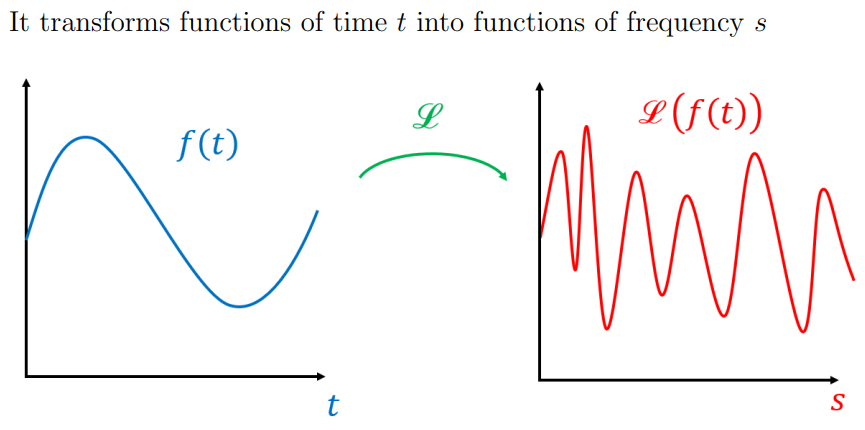
\includegraphics{Images/laplace.png}

\subsection*{Part II - Examples}
Example 1: $\mathcal{L}\{1\}$
\[\mathcal{L}\{1\} = \int_0^{\infty} 1e^{-st} \; dt = \int_0^{\infty} e^{st} \; dt = \left[\frac{e^{-st}}{-s}\right]_0^{\infty} = 0 + \frac{1}{s} = \boxed{\frac{1}{s}}\]

Example 2: $\mathcal{L}\{e^2t\}$
\[\mathcal{L}\{e^2t\} = \int_0^\infty e^(2- s) t\; dt = \left[\frac{e^{(2 - s)t}}{2 -s}\right]_0^\infty = 0 - \frac{1}{2 - s} = \boxed{\frac{1}{2 - s}}\]

\textbf{FACT:}
\[\boxed{\mathcal{L}\{e^{at}\} = \frac{1}{s - a} \quad (\text{if } s > a)}\]

Example 4: $\mathcal{L}\{\cos(2t)\}$ and $\mathcal{L}\{\sin (2t)\}$
\[\mathcal{L}\{\cos(2t)\} = \int_0^\infty \cos (2t) e^{-st}\; dt \]

Trick:
\[\mathcal{L}\{e^{(2t)i}\} = \mathcal{L}\{\cos (2t) + i \sin (2t)\} = \mathcal{L}\{\cos (2t)\} + i \mathcal{L}\{\sin (2t)\}\]

Then, 
\[\mathcal{L}\{e^{(2t)i}\} = \mathcal{L}\{e^{(2i)t}\} = \frac{1}{s - 2i} = \frac{s + 2i}{s^2 + 4} = \left(\frac{s}{s^2 + 4}\right) + i\left(\frac{2}{s^2 + 4}\right)\]

So,
\[\L{\cos(2t)} = \frac{s}{s^2 + 4}\]
\[\L{\sin(2t)} = \frac{2}{s^2 + 4}\]

\textbf{FACT:}
\[\boxed{\L{\cos(at)} = \frac{s}{s^2 + a^2} \quad \quad \L{\sin (at)} = \frac{a}{s^2 + a^2}}\]

Example 5: $\L{2 \sin (3t) + 4e^{5t}}$
\[= 2 \L \sin(3t) + 4 \L{e^5t} = \boxed{\frac{6}{s^2 + 9} + \frac{4}{s - 5}}\]

Example 6: $\L{U_2(t)}$
\[U_2(t) = \begin{cases}
    0 \quad t < 2\\
    1 \quad t \geq 2
\end{cases}\]
"The Heaviside function at 2" - used for unit impulse, etc. 

\[\L{U_2(t)} = \int_0^\infty U_2(t) e^{-st} \; dt =  \int_0^2 0 e^{-st} \; dt + \int_2^\infty 1 e^{-st} = \left[\frac{e^{st}}{-s}\right]_2^\infty = \boxed{\frac{e^{-2s}}{s}}\]

Example 7: Which function has laplace transform 
\[\frac{2}{s + 1} - \frac{4}{s - 3}\] 

\[= 2\L{e^{-t}} - 4 \L{e^{3t}} = \boxed{\L{2e^{-t} - 4e^{3t}}}\]

\subsection*{Part III - Tabular Integration}
Example 8: $\L{t^3} = \int_0^\infty t^3 \, e^{-st} \; dt$

Solution:
\[\begin{array}{c c c c}
    + & t^3 & & e^{-st}\\
    - & 3t^2 & \searrow  & e^{-st} / (-s)\\
    + & 6t & \searrow  & e^{-st} / (-s)^2\\
    - & 6 & \searrow  & e^{-st} / (-s)^3\\
    + & 0 & \searrow  & e^{-st} / (-s)^4\\
\end{array}\]

\[\implies \left[t^3 \left(\frac{e^{-st}}{-s}\right) - 3t^3 \left(\frac{e^{-st}}{(-s)^2}\right) + 6t \left(\frac{e^{-st}}{(-s)^3}\right) - 6 \left(\frac{e^{-st}}{(-s)^4}\right)\right]_0^\infty\] 
\[= 0 - (\frac{-6}{s^4}) = \boxed{\frac{6}{s^4}}\]

\textbf{FACT:}
\[\boxed{\L{t^n} = \frac{n!}{s^{n+1}}}\]

\section{Lecture Nov 30: Initial Value Problems}
\subsection*{Part I - Laplace Miracle}
Review:
\[\L{f(t)} = \int_0^\infty f(t) e^{-st} \; dt\]

Laplace miracle:
\[\L{f'(t)} = s\L{f(t)} - f(0)\]
Importantly, this turns differentiation into multiplication! This can obviously be used to turn differential equations into alegebraic equations 

Also, 
\[\L{f''(t)} = \L{(f'(t))'} = s\L{f'} - f'(0) = s^2 \L{f} - sf(0) - f'(0)\]

Proof: 
\[\L{f'(t) = \int_0^\infty  f'(t) \, e^{-st}\; dt}\]
Integrating by parts,
\[= \left[f(t) e^{-st}\right]_0^\infty - \int_0^\infty f(t) (-s)e^{-st} \; dt \]
\[= 0 - f(0) e^{-s (0)} + s \int_0^\infty f(t) e^{-st}\; dt\]
\[= s\L{f(t)} - f(0)\]

\subsection*{Part II - Applications to ODEs}
Example 1: Solve
\[\begin{cases}
    y'' - 5y' + 6y = 0\\
    y(0) = 4\\
    y'(0) = 9
\end{cases}\]

Solution:
\begin{enumerate}
    \item Take Laplace
    \[\L{y'' - 5y' + 6y} = \L{0}\]
    \[\L{y''} - 5\L{y'} + 6\L{y} = 0\]
    \[s^2\L{y} - sy(0) - y'(0) - 5s\L{y} - 5y(0) + 6\L{y} = s^2\L{y} - 4s - 9 - 5s\L{y} + 20 + 6\L{y} = 0\]
    \[= (s^2 - 5s + 6)s^2\L{y} - 4s - 9 + 20 = 0\]
    \[\L{y} = \frac{4s - 11}{s^2 - 5s + 6}\]

    Note that the denominator is the auxiliary equation!

    \item Use partial fractions
    \[\frac{4s - 11}{s^2 - 5s + 6} = \frac{4s - 11}{(s - 2)(s - 3)} = \frac{A}{s-2} + \frac{B}{s - 3}\]
    \[\frac{A(s-3) + B(s-2)}{s^2 - 5s + 6} = \frac{(A+B)s - 3A - 2B}{s^2 - 5s + 6}\]
    \[\begin{cases}
        A + B = 4\\
        -3A - 2B = -11
    \end{cases} \implies -3(4 - B) - 2B = -11 \implies B = 1, \; A = 3\]  
   
    \item Inverse laplace 
    So finally, 
    \[\L{y} = \frac{3}{s-2} + \frac{1}{s - 3}\]
    and 
    \[\boxed{y = 3e^{2t} + e^{3t}}\]
\end{enumerate}

Example 2: Solve 
\[y'' + y = -9\sin (2t)\\
y(0) = 2\\
y'(0) = 10\]

Solution:
\[(s^2 \L{y} - sy(0) - y'(0) + \L{y} = -9 \left(\frac{2}{s^2 + 4}\right))\]
\[(s^2 + 1) \L{y} - 2s - 10 = -9 \left(\frac{2}{s^2 + 4}\right) \]
\[\L{y} = \frac{-18 + (2s + 10)(s^2 + 4)}{(s^2 + 4)(s^2 + 1)}\]

Partial fractions:
\[\L{y} = \frac{2s^3 + 10s^2 + 8s + 22}{(s^2 + 4)(s^2 + 1)} = \frac{As + B}{(s^2 + 1)} + \frac{Cs + D}{(s^2 + 4)}\]
\[= \frac{(As + B)(s^2 + 4) + (Cs + D)(s^2 + 1)}{(s^2 + 4)(s^2 + 1)}\]
\[= \frac{As^3 + 4As + Bs^2 + 4B + Cs^3 + Cs + Ds^2 + D}{(s^2 + 4)(s^2 + 10)}\] 
\[= \frac{(A + C)s^3 + (B + D)s^2 + (4A + C)s + (4B + D)}{(s^2 + 4)(s^2 + 10)}\]
\[\begin{cases}
    A + C = 2\\
    B + D = 10\\
    4A + C = 8\\
    4B + D = 22
\end{cases} \implies \begin{cases}
    4(2 - C) + C = 8\\
    4(10 - D) + D = 22
\end{cases} = \begin{cases}
    -3C = 0\\
    -3D = -18
\end{cases} \implies \begin{cases}
    A = 2\\
    B = 4\\
    C = 0\\
    D = 6
\end{cases}\]

So, 
\[\L{y} = \frac{2s + 4}{(s^2 + 1)} + \frac{6}{(s^2 + 4)}\]
\[ = 2 \left(\frac{s}{s^2 + 1}\right) + 4\left(\frac{1}{s^2 + 1}\right) + 3\left(\frac{2}{s^2 + 4}\right)\]
\[\L{y} = \L{2\cos t + 4\sin t + 3 \sin(2t)}\]
\[\boxed{y = 2\cos t + 4\sin t + 3\sin(2t)}\]

\section{Lecture Dec 2: Step Functions (I)}
\subsection*{Part I - Step Functions}
Definition of Heaviside at 3:
\[U_3(t) = \begin{cases}
    0 \quad t < 3\\
    1 \quad t \geq 3
\end{cases}\]

\textbf{FACT:}
\[\L{U_n(t)} = \frac{e^{-ns}}{s}\]

Example 1: Find $\L{f(t)}$ where 
\[f(t) = \begin{cases}
    2 \quad 0 \leq t < 4\\
    5 \quad 4 \leq t < 7\\
    -1 \quad 7 \leq t < 9\\
    1 \quad t \geq 9\\
\end{cases}\]

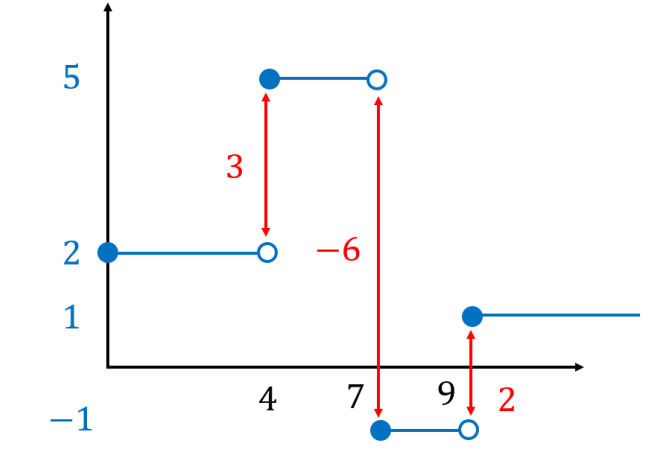
\includegraphics{Images/heaviside.png}

Solution:
Write f in terms of $U_c$
\[f(t) = 2 + 3U_4(t) - 6U_7(t) + 2U_9(t)\]
\[\boxed{\L{f(t)} = \frac{2}{s} + \frac{3e^{-4s}}{s} - \frac{6e^{-7s}}{s} + \frac{2e^{-9s}}{s}}\]

\subsection*{Part II - More general jumps}
\textbf{FACT:}
\[\L{t^n} = \frac{n!}{s^{n+1}}\]

Example 2: Find $\L{g(t)}$ where 
\[g(t) = \begin{cases}
    0 \quad t < 2\\
    (t - 2)^2 \quad t \geq 2
\end{cases}\]

Solution:
\[g(t) = (t - 2)^2 U_2(t)\]

Notice that g is of the form $g(t) = f(t - 2)U_2(t)$ where $f(t) = t^2$

\textbf{FACT:}
\[\L{f(t - 2)U_2(t)} = e^{-2s} \L{f(t)}\]
Note that the shift and the location of the heaviside must be the same  

Here, 
\[\L{g(t)} = \L{(t - 2)^2 U_2(t) = \boxed{\frac{2e^{-2s}}{s^3}}}\]

Example 3: Find $\L{g(t)}$ where 
\[g(t) = \begin{cases}
    1 \quad t < 5\\
    t - 4 \quad 5 \leq t < 10\\
    6 \quad t \geq 10
\end{cases}\]
\[g(t) = 1 + (t- 4 - 1)U_5(t) + (6 - (t - 4))U_{10}(t) = 1 + (t - 5)U_5(t) - (t - 10)U_10(t)\]
\[\L{g(t)} = 1 + e^{-5s}\left(\frac{1}{s^2}\right) - e^{-10s}\left(\frac{1}{s^2}\right) = \boxed{1 + \frac{e^{-5s}}{s^2} - \frac{e^{-10s}}{s^2}}\]

Example 4: Find the function whose laplace transform is 
\[\L{f(t)} = e^{-5s} \left(\frac{6}{s^4}\right) = g(t - 5) \L{g(t)} \]
\[\boxed{f(t) = (t - 5)^3 U_5(t)}\]

Example 5: Find the function whose laplace is 
\[\L{f(t)} = \frac{1}{s^2} + \left(\frac{s}{s^2 + 4}\right) e^{-3s}\]
\[\boxed{f(t) = t + U_3(t)\cos(2(t - 3))}\]

\subsection*{Part III - Shifting}
Example 6: $\L{e^{3t} \cos (2t)}$
Start with 
\[\L{\cos(2t)} = \frac{s}{s^2 + 4}\]

\textbf{FACT:}
\[\boxed{\L{e^{3t} \cos(2t)} = \frac{s - 3}{(s - 3)^2 + 4}}\]

Example 7: $\L{t^2 e^{-t}}$
\[\L{t^2} = \frac{2!}{s^3} = \frac{2}{s^3}\]
\[\boxed{\L{t^2 e^{-t}} = \frac{2}{(s + 1)^3}}\]

Example 8: Find a function whose laplace transform is 
\[\L{f(t)} = \frac{1}{(s- 2)^2 + 1}\]

Solution:
\[\L{\sin(t)} = \frac{1}{s^2 + 1}\]
So, 
\[\boxed{f(t) = e^{2t} \sin t}\]

Example 9: Find a function whose laplace transform is 
\[\L{f(t)} = \frac{6}{(s + 3)^4}\]
\[\boxed{f(t) = t^3e^{-3t}}\]

\section{Lecture Dec 5: Step Functions (II)}
\subsection*{Part I - More Practice}
Example 1: Find a function while laplace transform is 
\[\L{f(t)} = \frac{s}{s^2 - 6s + 13}\]

Solution:
Complete the square
\[\frac{s}{s^2 - 6s + 13} = \frac{s}{(s-3)^2 + 4} = \frac{s- 3}{(s-3)^2} + \frac{3}{(s-3)^2 + 4}\]

This is a shifted version of 
\[\frac{s- 3}{(s-3)^2} + \frac{3}{(s-3)^2 + 4} \implies \L{\cos (2t) + \frac{3}{2} \sin (2t)}\]

\[\boxed{f(t) = e^{3t}\left(\cos (2t) + \frac{3}{2} \sin (2t)\right)}\]

\subsection*{Part II - Putting everything together}
Example 2: Find a function whose laplace transform is 
\[\L{f(t)} = \frac{3(s - 2)e^{-3s}}{s^2 - 4s + 5}\]

Solution:
\[\frac{3(s - 2)e^{-3s}}{s^2 - 4s + 5} = e^{-3s} \left(\frac{3(s - 2)}{(s- 2)^2 + 1}\right)\]

\[ = e^{-3s} \L{3e^{2t}cos(t)} = \L{3e^{2(t - 3)} \cos(t- 3) U_3(t)}\]
\[\boxed{f(t) = 3e^{2(t - 3)} \cos(t- 3) U_3(t)}\]

\subsection*{Part III - ODE with Jumps}
Example 3: Solve the ODE 
\[\begin{cases}
    y'' + 4y = f(t)\\
    y(0) = 0\\
    y'(0) = 0
\end{cases} \quad f(t) = \begin{cases}
    0 \quad 0 \leq t < 5\\
    4t - 20 \quad 5 \leq t \leq 10\\
    20 \quad t \geq 10
\end{cases}\]

The function:
\[f(t) = (4t - 20)U_5(t) + (40 - 4t)U_{10}(t) = 4(t- 5)U_5 - 4(t - 10)U_{10}\]

\[\L{f(t)} = \L{4(t- 5)U_5} - \L{4(t - 10)U_{10}} = \frac{4}{s^2} \left(e^{-5s} - e^{-10s}\right)\]

The ODE:
\[\L{y''} + 4\L{y} = \L{f(t)}\]
\[s^2 \L{y} - sy(0) - y'(0) + 4\L{y} = \frac{4}{s^2} \left(e^{-5s} - e^{-10s}\right)\]
\[(s^2 + 4)\L{y} = \frac{4}{s^2} \left(e^{-5s} - e^{-10s}\right)\]
\[\L{y} = \frac{4}{s^2(s^2 + 4)}\left(e^{-5s} - e^{-10s}\right)\]

Partial Fractions:
Since $\frac{1}{s^2}$ is repeated, we guess 
\[\frac{4}{s^2(s^2 + 4)} = \frac{A}{s} + \frac{B}{s^2} + \frac{Cs + D}{s^2 + 4}\]
\[\implies \begin{cases}
    A + C = 0\\
    B + D = 0\\
    4A = 0\\
    4B = 4
\end{cases} \implies \begin{cases}
    A = 0\\
    B = 1\\
    C = 0\\
    D = -1
\end{cases}\]

\[\frac{4}{s^2(s^2 + 4)} = \frac{1}{s^2} - \frac{1}{s^2 + 4}\]
\[\L{y} = \left(\frac{1}{s^2} - \frac{1}{s^2 + 4}\right)\left(e^{-5s} - e^{-10s}\right)\]
\[= \L{t - \frac{1}{2}\sin(2t)} \left(e^{-5s} - e^{-10s}\right)\]
\[= \L{\left(t - 5 - \frac{1}{2}\sin(2t - 10)\right)U_5(t) - \left(t - 10 - \frac{1}{2}\sin(2t - 20)\right)U_{10}(t)} \]
\[\boxed{y = \left(t - 5 - \frac{1}{2}\sin(2t - 10)\right)U_5(t) - \left(t - 10 - \frac{1}{2}\sin(2t - 20)\right)U_{10}(t)}\]

\subsection*{Part IV - ODE with Shifts}
Example 4: 
\[\begin{cases}
    y'' + 4y' + 5y = f(t)\\
    y(0) = 0\\
    y'(0) = 0
\end{cases}\quad f(t) = \begin{cases}
    0 \quad 0 \leq t < 5\\
    5 \quad 5 \leq t < 20\\
    0 \quad t \geq 20
\end{cases}\]

\[f(t) = 5U(t) - 5U_{20}(t)\]
\[\L{f(t)} = \left(\frac{5}{s}\right)e^{-5s} - \left(\frac{5}{s}\right)e^{-20s}\]

\[\L{y''} + 4\L{y'} + 5\L{y} = \L{f(t)}\]
\[s^2 \L{y} + 4s\L{y} + 5\L{y} = \frac{5}{2}(e^{-5s} - e^{-20s})\]
\[(s^2 + 4s + 5)\L{y} = \frac{5}{2}(e^{-5s} - e^{-20s})\]
\[\L{y} = \frac{5}{s(s^2 + 4s + 5)}(e^{-5s} - e^{-20s})\]
\[\frac{5}{s(s^2 + 4s + 5)} = \frac{A}{s} + \frac{Bs + C}{s^2 + 4s + 5}\]
\[\begin{cases}
    A + B = 0\\
    4A + C = 0\\
    5A = 5
\end{cases} implies \begin{cases}
    A = 1\\
    B = -1\\
    C = -4
\end{cases}\]

\[\frac{5}{s(s^2 + 4s + 5)} =\frac{1}{s} + \frac{-s - 4}{s^2 + 4s + 5}\]

\[\L{y} = \left(\frac{1}{s} + \frac{-s - 4}{s^2 + 4s + 5}\right)(e^{-5s} - e^{-20s})\]
\[\frac{1}{s} = \L{1}\]

\[\frac{s + 4}{s^2 + 4s + 5} = \frac{s + 2 + 2}{(s + 2)^2 + 1} = \frac{s + 2}{(s+ 2^2 +1)} + \frac{2}{(s+2)^2 + 1}\]
\[ = \L{e^{-2t} (\cos(t) + 2\sin(t))}\]

\[\L{y} = \L{1 - e^{-2t} (\cos(t) + 2\sin(t))}(e^{-5s} - e^{-20s})\] 

\begin{empheq}[box=\fbox]{align*}
    y &= h(t - 5)U_5(t) - h(t - 20)U_{20}(t)\\
    h(t) &= 1 - e^{-2t} \cos t - 2e^{-2t} \sin t
\end{empheq}

\section{Lecture Dec 7: Dirac Delta}
\subsection*{Part I: Dirac and Roll}
\textbf{FACT:} There is a distribution $\delta(t)$ such that:
\begin{enumerate}
    \item $\delta(t) = 0$ except at $t = 0$ where $\delta(t) = \infty$
    \item $\int_{-\infty}^{\infty} \delta(t) = 1$
\end{enumerate}

\subsection*{Part II - Dirac Delta Laplace Transform}
\textbf{FACT:} For \emph{any} function $f(t)$, 
\[\int_0^{\infty} \delta(t) \, f(t) \; dt = f(0)\]
Using this property, 
\[\boxed{\L{\delta (t)} = 1}\]
Why?
\[\L{\delta (t)} = \int_0^{\infty}\delta(t)\; e^{-st}\; dt = f(0) = e^{-s(0)} = 1\]

Similarly, $\delta(t - 3)$ is a Dirac Delta with its spike at $t = 3$

\textbf{FACT:}
\[\L{\delta(t - c) = e^{-cs}}\]

Example 1:
\[\L{4\delta(t) - 2\delta(t - 3) + 5\delta(t - 6)} = 4 - 2e^{-3s} + 5e^{-6s}\]

\subsection*{Part III - ODE with Dirac Delta}
Example 2: 
\[\begin{cases}
    y'' + 4y' + 5y = \delta(t - 5)\\
    y(0) = 0\\
    y'(0) = 0
\end{cases}\]

\[\L{y''} + 4\L{y'} + 5\L{y} = \L{\delta (t - 5)}\]
\[s^2 \L{y} + 4s\L{y} + 5\L{y} = e^{-5s}\]
\[\L{y} = \frac{e^{-5s}}{s^2 - 4s + 5}\]
\[\L{y} = \L{e^{2t\sin(t)}} e^{-5s} = \L{e^{2(t- 5) \sin(t - 5) U_5(t)}}\]
\[y = e^{2(t- 5) \sin(t - 5) U_5(t)}\]

Example 3: 
\[\begin{cases}
    y'' + 3y' + 2y = -12\delta(t - 3)\\
    y(0) = 2\\
    y'(0) = -3
\end{cases}\]

Solution:
\[\L{y''} + 3\L{y'} + 2\L{y} = -12\L{\delta(t- 3)}\]
\[(s^2 + 3s + 2) \L{y} = (2s + 3) -12e^{-3s}\]
\[\L{y} =\frac{2s + 3}{s^2 + 3s +2} - \frac{12}{s^2 + 3s +2}e^{-3s}\]
Partial fractions:
First term: 
\[\frac{2s + 3}{(s + 1)(s + 2)} = \frac{A}{s+1} + \frac{B}{s + 2}\]
\[\begin{cases}
    A + B = 2\\
    2A + B = 3
\end{cases} \implies A = 1, \quad B = 1\]

Second term: 
\[\frac{-12}{s^2 + 3s+2} = \frac{A}{s+ 1} + \frac{B}{s+2}\]
\[\begin{cases}
    A+B = 0\\
    2A + B = -12
\end{cases} \implies A = -12 \quad B = 12\]

Putting together:
\begin{align*}
    \L{y} &= \frac{2s + 3}{s^2 + 3s +2} - \frac{12}{s^2 + 3s +2}e^{-3s}\\
    &= \left(\frac{1}{s + 1} + \frac{1}{s + 2}\right) + \left(\frac{-12}{s + 1} + \frac{12}{s + 2}\right)e^{-3s}\\
    &= \L{e^{-t} + e^{-2t}} + \L{-12e^{-t} + 12e^{-2t}}e^{-3s}\\
    &= \L{e^{-t} + e^{-2t} + (-12e^{-(t-3)} + 12e^{-2(t-3)})U_3(t)}
\end{align*}
\[\boxed{y= e^{-t} + e^{-2t} + (-12e^{-(t-3)} + 12e^{-2(t-3)})U_3(t)}\]
\end{document}   